\documentclass{uai2023} % for initial submission
% \documentclass[accepted]{uai2023} % after acceptance, for a revised
                                    % version; also before submission to
                                    % see how the non-anonymous paper
                                    % would look like
%% There is a class option to choose the math font
% \documentclass[mathfont=ptmx]{uai2023} % ptmx math instead of Computer
                                         % Modern (has noticable issues)
% \documentclass[mathfont=newtx]{uai2023} % newtx fonts (improves upon
                                          % ptmx; less tested, no support)
% NOTE: Only keep *one* line above as appropriate, as it will be replaced
%       automatically for papers to be published. Do not make any other
%       change above this note for an accepted version.

%% Choose your variant of English; be consistent
\usepackage[american]{babel}
% \usepackage[british]{babel}

%% Some suggested packages, as needed:
\usepackage{natbib} % has a nice set of citation styles and commands
    \bibliographystyle{plainnat}
    \renewcommand{\bibsection}{\subsubsection*{References}}
% \usepackage{mathtools} % amsmath with fixes and additions
% \usepackage{siunitx} % for proper typesetting of numbers and units
\usepackage{booktabs} % commands to create good-looking tables
% \usepackage{tikz} % nice language for creating drawings and diagrams

\relax % Controls
    \newif\ifmarginprooflinks
    	\marginprooflinkstrue
    	% \marginprooflinksfalse

\relax % Bibliography, etc
	\usepackage[american]{babel}
	\usepackage{csquotes}
	\usepackage[backend=biber, style=authoryear]{biblatex}
	\DeclareLanguageMapping{american}{american-apa}
	% \usepackage[backend=biber,style=authoryear,hyperref=true]{biblatex}
	% \addbibresource{refs.bib}
	% \addbibresource{conf.bib}

	\DeclareFieldFormat{citehyperref}{%
	  \DeclareFieldAlias{bibhyperref}{noformat}% Avoid nested links
	  \bibhyperref{#1}}

	\DeclareFieldFormat{textcitehyperref}{%
	  \DeclareFieldAlias{bibhyperref}{noformat}% Avoid nested links
	  \bibhyperref{%
	    #1%
	    \ifbool{cbx:parens}
	      {\bibcloseparen\global\boolfalse{cbx:parens}}
	      {}}}

	\savebibmacro{cite}
	\savebibmacro{textcite}

	\renewbibmacro*{cite}{%
	  \printtext[citehyperref]{%
	    \restorebibmacro{cite}%
	    \usebibmacro{cite}}}

	\renewbibmacro*{textcite}{%
	  \ifboolexpr{
	    ( not test {\iffieldundef{prenote}} and
	      test {\ifnumequal{\value{citecount}}{1}} )
	    or
	    ( not test {\iffieldundef{postnote}} and
	      test {\ifnumequal{\value{citecount}}{\value{citetotal}}} )
	  }
	    {\DeclareFieldAlias{textcitehyperref}{noformat}}
	    {}%
	  \printtext[textcitehyperref]{%
	    \restorebibmacro{textcite}%
	    \usebibmacro{textcite}}}

	\DeclareCiteCommand{\brakcite}
	  {\usebibmacro{prenote}}
	  {\usebibmacro{citeindex}%
	   \printtext[bibhyperref]{[\usebibmacro{cite}]}}
	  {\multicitedelim}
	  {\usebibmacro{postnote}}

\relax % Standard Packages
    \usepackage[dvipsnames]{xcolor}
    % \usepackage[utf8]{inputenc}
    \usepackage{mathtools}
    \usepackage{amssymb}
		\DeclareMathSymbol{\shortminus}{\mathbin}{AMSa}{"39}
    % \usepackage{parskip}
    % \usepackage{algorithm}
    \usepackage{bbm}
	\usepackage{lmodern}
	% \usepackage{times}
    \usepackage{faktor}
    % \usepackage{booktabs}
	% \usepackage[margin=1in]{geometry}
    \usepackage{graphicx}
    \usepackage{scalerel}
    \usepackage{enumitem}
    \usepackage{nicefrac}\let\nf\nicefrac

    % \usepackage{color}
    %\usepackage{stmaryrd}
    \usepackage{hyperref} % Load before theorems...
        \hypersetup{colorlinks=true, linkcolor=blue!75!black, urlcolor=magenta, citecolor=green!50!black}

\usepackage{tikz}
	\usetikzlibrary{positioning,fit,calc, decorations, arrows, shapes, shapes.geometric}
	\usetikzlibrary{cd}

	%%%%%%%%%%%%
	\tikzset{AmpRep/.style={ampersand replacement=\&}}
	\tikzset{center base/.style={baseline={([yshift=-.8ex]current bounding box.center)}}}
	\tikzset{paperfig/.style={center base,scale=0.9, every node/.style={transform shape}}}

	% Node Stylings
	\tikzset{dpadded/.style={rounded corners=2, inner sep=0.7em, draw, outer sep=0.3em, fill={black!50}, fill opacity=0.08, text opacity=1}}
	\tikzset{dpad0/.style={outer sep=0.05em, inner sep=0.3em, draw=gray!75, rounded corners=4, fill=black!08, fill opacity=1, align=center}}
	\tikzset{dpadinline/.style={outer sep=0.05em, inner sep=2.5pt, rounded corners=2.5pt, draw=gray!75, fill=black!08, fill opacity=1, align=center, font=\small}}

 	\tikzset{dpad/.style args={#1}{every matrix/.append style={nodes={dpadded, #1}}}}
	\tikzset{light pad/.style={outer sep=0.2em, inner sep=0.5em, draw=gray!50}}

	\tikzset{arr/.style={draw, ->, thick, shorten <=3pt, shorten >=3pt}}
	\tikzset{arr0/.style={draw, ->, thick, shorten <=0pt, shorten >=0pt}}
	\tikzset{arr1/.style={draw, ->, thick, shorten <=1pt, shorten >=1pt}}
	\tikzset{arr2/.style={draw, ->, thick, shorten <=2pt, shorten >=2pt}}

	\newcommand\cmergearr[5][]{
		\draw[arr, #1, -] (#2) -- (#5) -- (#3);
		\draw[arr, #1, shorten <=0] (#5) -- (#4);
		}
	\newcommand\mergearr[4][]{
		\coordinate (center-#2#3#4) at (barycentric cs:#2=1,#3=1,#4=1.2);
		\cmergearr[#1]{#2}{#3}{#4}{center-#2#3#4}
		}
	\newcommand\cunmergearr[5][]{
		\draw[arr, #1, -, shorten >=0] (#2) -- (#5);
		\draw[arr, #1, shorten <=0] (#5) -- (#3);
		\draw[arr, #1, shorten <=0] (#5) -- (#4);
		}
	\newcommand\unmergearr[4][]{
		\coordinate (center-#2#3#4) at (barycentric cs:#2=1.2,#3=1,#4=1);
		\cunmergearr[#1]{#2}{#3}{#4}{center-#2#3#4}
		}

\usepackage{amsthm,thmtools} % Theorem Macros
	\usepackage[noabbrev,nameinlink,capitalize]{cleveref}
    \theoremstyle{plain}
    \newtheorem{theorem}{Theorem}
	\newtheorem{coro}{Corollary}[theorem]
    \newtheorem{prop}[theorem]{Proposition}
    \newtheorem{conj}[theorem]{Conjecture}
    \newtheorem{claim}{Claim}
    \newtheorem{remark}{Remark}
    \newtheorem{lemma}[theorem]{Lemma}
    \theoremstyle{definition}
    % \newtheorem{defn}{Definition}
    % \declaretheorem[name=Definition]{defn}
    \declaretheorem[name=Definition, qed=$\square$]{defn}
    \declaretheorem[name=Example, qed=$\triangle$]{example}

    \definecolor{openQcolor}{rgb}{0.9,0.2,0.9}
    \declaretheorem[preheadhook=\color{openQcolor},name=Open Question]{openQ}

	\crefname{defn}{Definition}{Definitions}
	\crefname{prop}{Proposition}{Propositions}
    \crefname{issue}{Issue}{Issues}

\relax %%%%%%%%% GENERAL MACROS %%%%%%%%
    \let\Horig\H
	\let\H\relax
	\DeclareMathOperator{\H}{\mathrm{H}} % Entropy
	\DeclareMathOperator{\I}{\mathrm{I}} % Information
	\DeclareMathOperator*{\Ex}{\mathbb{E}} % Expectation
	\DeclareMathOperator*{\EX}{\scalebox{1.5}{$\mathbb{E}$}}
    \newcommand{\ifrac}[2]{{#1}/{#2}}
    
    % \DeclareMathOperator{\argmin}{\arg\min}
    \DeclareMathOperator*{\argmin}{\arg\!\min}
    \DeclareMathOperator*{\argmax}{\arg\!\max}

    \newcommand{\mat}[1]{\mathbf{#1}}
    \DeclarePairedDelimiterX{\infdivx}[2]{(}{)}{%
		#1\;\delimsize\|\;#2%
	}
	\newcommand{\thickD}{I\mkern-8muD}
	\newcommand{\kldiv}{\thickD\infdivx}
	\newcommand{\tto}{\rightarrow\mathrel{\mspace{-15mu}}\rightarrow}

	\newcommand{\datadist}[1]{\Pr\nolimits_{#1}}
	% \newcommand{\datadist}[1]{p_\text{data}}

	\makeatletter
	\newcommand{\subalign}[1]{%
	  \vcenter{%
	    \Let@ \restore@math@cr \default@tag
	    \baselineskip\fontdimen10 \scriptfont\tw@
	    \advance\baselineskip\fontdimen12 \scriptfont\tw@
	    \lineskip\thr@@\fontdimen8 \scriptfont\thr@@
	    \lineskiplimit\lineskip
	    \ialign{\hfil$\m@th\scriptstyle##$&$\m@th\scriptstyle{}##$\hfil\crcr
	      #1\crcr
	    }%
	  }%
	}
	\makeatother
	\newcommand\numberthis{\addtocounter{equation}{1}\tag{\theequation}}

\relax %%%%%%%%%   PDG  MACROS   %%%%%%%%
	\newcommand{\ssub}[1]{_{\!_{#1}\!}}
	% \newcommand{\bp}[1][L]{\mat{p}_{\!_{#1}\!}}
	% \newcommand{\bP}[1][L]{\mat{P}_{\!_{#1}\!}}
	\newcommand{\bp}[1][L]{\mat{p}\ssub{#1}}
	\newcommand{\bP}[1][L]{\mat{P}\ssub{#1}}
	\newcommand{\V}{\mathcal V}
	\newcommand{\N}{\mathcal N}
	\newcommand{\Ed}{\mathcal E}

    \newcommand{\balpha}{\boldsymbol\alpha}
    \newcommand{\bbeta}{\boldsymbol\beta}

	\DeclareMathAlphabet{\mathdcal}{U}{dutchcal}{m}{n}
	\DeclareMathAlphabet{\mathbdcal}{U}{dutchcal}{b}{n}
	\newcommand{\dg}[1]{\mathbdcal{#1}}
	\newcommand{\PDGof}[1]{{\dg M}_{#1}}
	\newcommand{\UPDGof}[1]{{\dg N}_{#1}}
	\newcommand\VFE{\mathit{V\mkern-4mu F\mkern-4.5mu E}}

	\newcommand\Inc{\mathit{Inc}}
	\newcommand{\IDef}[1]{\mathit{IDef}_{\!#1}}
	% \newcommand{\ed}[3]{%
	% 	\mathchoice%
	% 	{#2\overset{\smash{\mskip-5mu\raisebox{-3pt}{${#1}$}}}{\xrightarrow{\hphantom{\scriptstyle {#1}}}} #3} %display style
	% 	{#2\overset{\smash{\mskip-5mu\raisebox{-3pt}{$\scriptstyle {#1}$}}}{\xrightarrow{\hphantom{\scriptstyle {#1}}}} #3}% text style
	% 	{#2\overset{\smash{\mskip-5mu\raisebox{-3pt}{$\scriptscriptstyle {#1}$}}}{\xrightarrow{\hphantom{\scriptscriptstyle {#1}}}} #3} %script style
	% 	{#2\overset{\smash{\mskip-5mu\raisebox{-3pt}{$\scriptscriptstyle {#1}$}}}{\xrightarrow{\hphantom{\scriptscriptstyle {#1}}}} #3}} %scriptscriptstyle
	\newcommand{\ed}[3]{#2%
	  \overset{\smash{\mskip-5mu\raisebox{-1pt}{$\scriptscriptstyle
	        #1$}}}{\rightarrow} #3}

    \newcommand{\nhphantom}[2]{\sbox0{\kern-2%
		\nulldelimiterspace$\left.\delimsize#1\vphantom{#2}\right.$}\hspace{-.97\wd0}}
		% \nulldelimiterspace$\left.\delimsize#1%
		% \vrule depth\dp#2 height \ht#2 width0pt\right.$}\hspace{-.97\wd0}}
	\makeatletter
	\newsavebox{\abcmycontentbox}
	\newcommand\DeclareDoubleDelim[5]{
	    \DeclarePairedDelimiterXPP{#1}[1]%
			{% box must be saved in this pre code
				\sbox{\abcmycontentbox}{\ensuremath{##1}}%
			}{#2}{#5}{}%
		    %%% Correct spacing, but doesn't work with externalize.
			% {\nhphantom{#3}{##1}\hspace{1.2pt}\delimsize#3\mathopen{}##1\mathclose{}\delimsize#4\hspace{1.2pt}\nhphantom{#4}{##1}}
			%%% Fast, but wrong spacing.
			% {\nhphantom{#3}{~}\hspace{1.2pt}\delimsize#3\mathopen{}##1\mathclose{}\delimsize#4\hspace{1.2pt}\nhphantom{#4}{~}}
			%%% with savebox.
		    {%
				\nhphantom{#3}{\usebox\abcmycontentbox}%
				\hspace{1.2pt} \delimsize#3%
				\mathopen{}\usebox{\abcmycontentbox}\mathclose{}%
				\delimsize#4\hspace{1.2pt}%
				\nhphantom{#4}{\usebox\abcmycontentbox}%
			}%
	}
	\makeatother
	\DeclareDoubleDelim
		\SD\{\{\}\}
	\DeclareDoubleDelim
		\bbr[[]]
	% \DeclareDoubleDelim
	% 	\aar\langle\langle\rangle\rangle
	\makeatletter
	\newsavebox{\aar@content}
	\newcommand\aar{\@ifstar\aar@one@star\aar@plain}
	\newcommand\aar@one@star{\@ifstar\aar@resize{\aar@plain*}}
	\newcommand\aar@resize[1]{\sbox{\aar@content}{#1}\scaleleftright[3.8ex]
		{\Biggl\langle\!\!\!\!\Biggl\langle}{\usebox{\aar@content}}
		{\Biggr\rangle\!\!\!\!\Biggr\rangle}}
	\DeclareDoubleDelim
		\aar@plain\langle\langle\rangle\rangle
	\makeatother


	% \DeclarePairedDelimiterX{\aar}[1]{\langle}{\rangle}
	% 	{\nhphantom{\langle}{#1}\hspace{1.2pt}\delimsize\langle\mathopen{}#1\mathclose{}\delimsize\rangle\hspace{1.2pt}\nhphantom{\rangle}{#1}}

\relax %%%%% restatables and links
	% \usepackage{xstring} % for expandarg
	\usepackage{xpatch}
	\makeatletter
	\xpatchcmd{\thmt@restatable}% Edit \thmt@restatable
	   {\csname #2\@xa\endcsname\ifx\@nx#1\@nx\else[{#1}]\fi}% Replace this code
	   % {\ifthmt@thisistheone\csname #2\@xa\endcsname\typeout{oiii[#1;#2\@xa;#3;\csname thmt@stored@#3\endcsname]}\ifx\@nx#1\@nx\else[#1]\fi\else\csname #2\@xa\endcsname\fi}% with this code
	   {\ifthmt@thisistheone\csname #2\@xa\endcsname\ifx\@nx#1\@nx\else[{#1}]\fi
	   \else\fi}
	   {}{\typeout{FIRST PATCH TO THM RESTATE FAILED}} % execute on success/failure
	\xpatchcmd{\thmt@restatable}% A second edit to \thmt@restatable
	   {\csname end#2\endcsname}
	   {\ifthmt@thisistheone\csname end#2\endcsname\else\fi}
	   {}{\typeout{FAILED SECOND THMT RESTATE PATCH}}

	% \def\onlyaftercolon#1:#2{#2}
	\newcommand{\recall}[1]{\medskip\par\noindent{\bf \Cref{thmt@@#1}.} \begingroup\em \noindent
	   \expandafter\csname#1\endcsname* \endgroup\par\smallskip}

   	\setlength\marginparwidth{1.55cm}
	\newenvironment{linked}[3][]{%
		\def\linkedproof{#3}%
		\def\linkedtype{#2}%
		% \reversemarginpar
		% \marginpar{%
		% \vspace{1.1em}
		% % \hspace{2em}
		% 	% \raggedleft
		% 	\raggedright
		% 	\hyperref[proof:\linkedproof]{%
		% 	\color{blue!50!white}
		% 	\scaleleftright{$\Big[$}{\,{\small\raggedleft\tt\begin{tabular}{@{}c@{}} proof of \\\linkedtype~\ref*{\linkedtype:\linkedproof}\end{tabular}}\,}{$\Big]$}}
		% 	}%
        % \restatable[#1]{#2}{#2:#3}\label{#2:#3}%
		\ifmarginprooflinks
		\marginpar{%
			% \vspace{-3em}% %% for bottom
			\vspace{1.5em}
			\centering%
			\hyperref[proof:\linkedproof]{%
            % \hyperref[proof:#3]{
			\color{blue!30!white}%
			\scaleleftright{$\Big[$}{\,\mbox{\footnotesize\centering\tt\begin{tabular}{@{}c@{}}
				% proof of \\\,\linkedtype~\ref*{\linkedtype:\linkedproof}
				link to\\[-0.15em]
				proof
			\end{tabular}}\,}{$\Big]$}}~
			}%
		\fi
        \restatable[#1]{#2}{#2:#3}\label{#2:#3}%
        }%
		{\endrestatable%
		}
	\makeatother
		\newcounter{proofcntr}
		\newenvironment{lproof}{\begin{proof}\refstepcounter{proofcntr}}{\end{proof}}

		\usepackage{cancel}
		\newcommand{\Cancel}[2][black]{{\color{#1}\cancel{\color{black}#2}}}

		\usepackage{tcolorbox}
		\tcbuselibrary{most}
		\tcolorboxenvironment{lproof}{
			% fonttitle=\bfseries,
			% top=0.5em,
			enhanced,
			parbox=false,
			boxrule=0pt,
			frame hidden,
			borderline west={4pt}{0pt}{blue!20!black!40!white},
			% coltext={blue!20!black!60!white},
			colback={blue!20!black!05!white},
			sharp corners,
			breakable,
			% bottomsep at break=4cm,
			% enlarge bottom at break by=-4cm,
			% topsep at break=3cm,
			% enlarge top at break by=-3cm
		}
		% \usepackage[framemethod=TikZ]{mdframed}
		% \surroundwithmdframed[ % lproof
		% 	   topline=false,
		% 	   linewidth=3pt,
		% 	   linecolor=gray!20!white,
		% 	   rightline=false,
		% 	   bottomline=false,
		% 	   leftmargin=0pt,
		% 	   % innerleftmargin=5pt,
		% 	   skipabove=\medskipamount,
		% 	   skipbelow=\medskipamount
		% 	]{lproof}
	%oli16: The extra space was because there was extra space in the paragraph, not
	%because this length was too big. By breaking arrays, everything will be better.
	\newcommand{\begthm}[3][]{\begin{#2}[{name=#1},restate=#3,label=#3]}

\relax %TODOs and footnotes
    \newcommand{\TODO}[1][INCOMPLETE]{{\centering\Large\color{red}$\langle$~\texttt{#1}~$\rangle$\par}}
    \newcommand{\dfootnote}[1]{%
        \let\oldthefootnote=\thefootnote%
        % \addtocounter{footnote}{-1}%
		\setcounter{footnote}{999}
        \renewcommand{\thefootnote}{\textdagger}%
        \footnote{#1}%
        \let\thefootnote=\oldthefootnote%
    }
	\newcommand{\dfootnotemark}{
		\footnotemark[999]
	}


% \usepackage[framemethod=TikZ]{mdframed}
% \colorlet{color1}{Emerald}
% \colorlet{color3}{color1>wheel,2,3}
% \colorlet{pinkish}{color3!25!magenta}
\definecolor{brownish}{rgb}{0.5, 0.2, 0.1}
% \newmdenv[roundcorner=5pt, 
%     backgroundcolor=brownish!20!white,
%     % frametitle={$\langle$under construction$\rangle$},
%     frametitle={$\langle$incomplete or buggy$\rangle$},
%     frametitlerule=false,
%     innertopmargin=3pt, frametitlebelowskip=1ex, frametitleaboveskip=1ex,
%     frametitlebackgroundcolor=brownish!40!white,
%     skipabove=1em,skipbelow=1em,
%     frametitlefont={\scshape},leftmargin=-10pt, rightmargin=-10pt]
% 		{wip}
\newtcolorbox{wip}{%
    colback=brownish!20!white,%
    % frametitle={$\langle$under construction$\rangle$},
    title={$\langle$under construction$\rangle$},%
    enhanced jigsaw,
    breakable,
    % frametitlerule=false,
    % innertopmargin=3pt, frametitlebelowskip=1ex, frametitleaboveskip=1ex,
    colframe=brownish!40!white,%
    % skipabove=1em,skipbelow=1em,
    % frametitlefont={\scshape},leftmargin=-10pt, rightmargin=-10pt
}
        
% \tcolorboxenvironment{example}{
% \newtcolorbox[use counter=example]{examplex}{
\newtcbtheorem[use counter=example]{examplex}{Example}{
        label type=example,
        fonttitle=\bfseries,
        % empty,
        enhanced jigsaw,
        % title={Example \thetcbcounter.},
        before=\par\medskip\noindent,
        % top=0.5em,
        % enhanced,
        parbox=false,
        % boxrule=0pt,
        % frame hidden,
        % borderline west={4pt}{0pt}{green!20!black!40!white},
        % coltext={blue!20!black!60!white},
        % colback={blue!20!black!05!white},
        colback=white,
        sharp corners,
        breakable,
        % bottomsep at break=4cm,
        % enlarge bottom at break by=-4cm,
        % topsep at break=3cm,
        % enlarge top at break by=-3cm
    }
    %
    {ex}


\makeatletter
\newcommand{\@minipagerestore}{\setlength{\parskip}{\medskipamount}}
\makeatother

\usepackage{xparse}
\let\realItem\item % save a copy of the original item
\makeatletter
\NewDocumentCommand\myItemboldperiod{ o }{%
   \IfNoValueTF{#1}%
      {\realItem}% add an item
      {\realItem[\textbf{#1.}]\def\@currentlabel{#1}%
        % \def\cref@currentlabel{#1}
        }% add an item and update label
}
\makeatother


% \usepackage{enumitem}
\newlist{URaxioms}{enumerate}{1}
\setlist[URaxioms]{
    resume,%
    label=\textbf{UR\arabic{*}.},
    % label=UR\arabic{*},
    ref={UR\arabic*},
    leftmargin=2cm,
    before=\let\item\myItemboldperiod,
    topsep=1ex
    }
% \crefname{URaxiomsi}{axiom}{axioms}
\crefname{URaxiomsi}{}{}
\newcommand\commentout[1]{}

% \addbibresource{conf.bib}

%% Provided macros
% \smaller: Because the class footnote size is essentially LaTeX's \small,
%           redefining \footnotesize, we provide the original \footnotesize
%           using this macro.
%           (Use only sparingly, e.g., in drawings, as it is quite small.)

%% additional macros
\newcommand{\ext}[1]{\overline #1} %  measures over phi
\newcommand{\Unif}{\mathrm{Unif}}

\newcommand\cofunc{commitment function}
\newcommand\confdom{\mathdcal C}
\newcommand\ZO{\mathrm{ZO}}
% \def\ZO{[0,1]}
\newcommand\Rplus{\mathbb R_+}
\newcommand\X{\mathcal X}

% \let\oldTheta\Theta
% \renewcommand\Theta{\mathdcal{\Theta}}

% \title{Measures of Confidence}
\title{%
    % Updating with Confidence
    Updating with Confidence
}

% The standard author block has changed for UAI 2022 to provide
% more space for long author lists and allow for complex affiliations
%
% All author information is authomatically removed by the class for the
% anonymous submission version of your paper, so you can already add your
% information below.

% Add authors
\author[1]{\href{mailto:<oer5@cornell.edu>?Subject=confidence-paper}{Oliver E Richardson}{}}
\author[1]{Joseph Y Halpern}
% Add affiliations after the authors
\affil[1]{%
    Computer Science Dept.\\
    Cornell University\\
    Ithaca, New York, USA
}

\begin{document}
\maketitle

\begin{abstract}
We introduce a new notion of confidence, which arises when learning or updating beliefs.
\end{abstract}

\section{Introduction}\label{sec:intro}
\def\stmt{$A$}
% \def\stmt{$\phi$}


\commentout{%oli-v1
	% The ability articulate a \emph{degree of confidence} is an important aspect of knowledge representation.
	The ability to articulate a \emph{degree of confidence} 
	% (or the opposite: a degree of uncertainty)
	is a critical aspect of representing knowledge.
	There are 
	% Correspondingly, there are
	many well-established ways to quantify (un)certinaty \parencite[\S2]{halpern2017reasoning},
		and chief among them is probability.
	While ``confidence'' can be coherently read in probabilistic terms,
		such usage may shadow another important concept.
	This paper details a different conception that arises when updating beliefs. 
	As we shall see, this notion of confidence
	complements traditional representations of uncertainty (such as probability), 
	and moreover unifies several different concepts across AI.
}

What should it mean to say that one has a high degree of confidence in a statement $\phi$?  It is often taken to mean that we think $\phi$ is likely. 
% This paper details a different conception that arises when updating beliefs. 
% As we shall see, this notion of confidence
% complements traditional representations of uncertainty (such as probability), 
Here we argue that there is a related but more useful conception of confidence that arises when updating---one that complements likelihood and, moreover, unifies several different concepts in the literature.
% Here we argue that there is a related but more useful way of defining confidence, which complements notions like probability and, moreover, unifies several different concepts in the literature.

% For us, confidence is a measure of trust (in incoming information), rather than of likelihood (of hypothetical information). 
% For us, confidence (in an input $\phi$) is a measure of \emph{trust}, rather than of likelihood; it quantifies seriously to take $\phi$ in updating one's beliefs.
%
%joe1:
% For us, the degree of confidence in $\phi$ is a measure of the degree
% to which we \emph{trust} $\phi$,
% rather than of the likelihood of $\phi$.  We formalize this by taking
% the degree of confidence to represent how seriously to take $\phi$
% when updating beliefs.
%
%oli1: with reference to your rewrite (above): I don't like the way the grammar 
% worked out; my lead-in "for us" muddies the "our confidence" part 
% that you wrote. Let me try to clean it up. 
%
For us, confidence is a measure of \emph{trust}, rather than likelihood.
In particular, the {degree of confidence} that one has in a piece of information $\phi$
%is a number  $\chi \in [\bot,\top]$ that 
quantifies how seriously to take $\phi$ in updating one's beliefs. 
%oli1:
% In the below, I replaced "0" and "1" with "no" and "full" because
% I want don't want to lock in the range [0,1] at this level of generality.
% More importantly, the second part about "taking \phi to be true" doesn't
% make as much sense in general, so I rephrased it.
%
% Thus, if we learn $\phi$ but have confidence 0 in it, it should not
% affect our beliefs at all, while if we have confidence 1 in $\phi$, we
% should update our beliefs by taking $\phi$ to be true; in a
% probabilistic setting, this amounts to conditioning on $\phi$. 
%
% Thus,
So at one extreme,
if we observe $\phi$ but have no confidence in it, 
% it should not affect our beliefs at all;
we should not change our beliefs at all;
at the other, if we have full confidence in $\phi$,
 we should fully incorporate it into our beliefs.
 
% , in some sense.
% In the setting where, our beliefs is a probability measure $\Pr$, and $\phi$ is an event, 
% In a probabilistic setting, we can capture an intermediate degree of
% If our belief state is a probability measure $\Pr$ and $\phi$ is an event, for example, then fully incorporating $\phi$ amounts to conditioning $\Pr$ on it.
\begin{example} \label{ex:prob-simple}
% Suppose, for example, that 
Suppose
% For example, if
our belief state is a probability measure, and $\phi$ is an event. 
% In this setting, 
% Here,
A full-confidence update then amounts to conditioning on $\phi$, after which $\phi$ has probability 1, and so cannot be further incorporated.
%oli1: changed from "the obvious way" to "an obvious way"
% In a probabilistic setting, we can capture an  intermediate degree of confidence by interpolating in the obvious way:
% In this case,
% we can also capture intermediate degrees of confidence in an obvious way:
We also have an obvious way to describe intermediate degrees of confidence:
if we learn $\phi$ with confidence
%oli1: now adding range here
% $\alpha$
$\alpha \in [0,1]$
% and start with a prior probability $\Pr$, then we end up with the
and start with prior probability $\Pr$, then we end up with the
%oli1: I agree that this notation is nicer, but these days it
% is also much less standard than p(X) and p(X|\phi). In particular,
% my ML friends who work with applied probability a lot do not understand
% how to parse  "\Pr | \phi". 
posterior $(1-\alpha)\Pr + \alpha (\Pr\mid \phi)$.
%
Thus, having high confidence in $\phi$ leads to posterior beliefs that give $\phi$
high
%oli1: I've seen a lot of statistics people make a big fuss about
% this being the wrong usage of the word "likelihood", which I've been
% told applies to evidence that is being conditioned on, and not to 
% events whose probability we're querying.  Now that we have a
% probability in scope, I'd prefer to avoid this fight by just saying:
%likelihood.
probability.
% But confidence and probability are not always so tightly coupled.
% Still, confidence and probability are quite different in general.
The converse is false, however, so
confidence and probability can be quite different.
% 
%oli1: the context here has been stripped; we're now missing how it might be possible to learn \phi with low confidence if we already assign it high probability.
% If we start out with a prior that gives $\phi$ high likelihood, and learn $\phi$ with low confidence, our posterior beliefs still give $\phi$ high likelihood.  
% We might also have a great deal of confidence in an observation of $\phi$  despite having a low prior belief in $\phi$.
If an untrusted source tells us $\phi$ which we already happen to believe, 
then our prior assigns $\phi$ high probability,
we learn $\phi$ with low confidence,
and our posterior beliefs still give $\phi$ high probability.  
% then we learn $\phi$ with low confidence, but both 
% Confidence is even easier to distinguish from prior probability: 
Confidence and prior probability are even more independent: 
if we learn a surprising fact $\phi$ from a trusted source, we have high confidence in $\phi$ despite it having low prior probability.
% This leads to an important observation: one's confidence in $\phi$ is not a feature of one's prior probability at all.
\end{example}

\commentout{
	In this context, 
	the confidence $\chi \in [0,1]$ has a clear interpretation as the ``fraction of the way towards full incorporation'',
	but in others,
	it may be 
	less clear what a number on this scale (say, $\chi{=}0.7$) means.
	% there is still a natural path from distrust to complete trust that is parameterized differently.
	% In other cases, there are other more natural ways to articulate one's confidence.
}

%oli1: something bothers me about starting a paragraph with "but", 
% especially without directly pushing off of something concrete about the
% way the previous sentence ended.
% But confidence can be applied far more broadly.
% This notion of confidence applies far more broadly. 
This notion of confidence applies far more broadly.
% Here is an example that has similar 
% We now give a quite different ,
We now give an example with the same critical elements,
but a very different flavor.
% of a very different flavor, 
% in which confidence is measured differently.

\begin{example}\label{ex:classifier}
Consider a neural network, whose ``belief state'' is a setting of weights.
% $ \in \mathbb R^n$.
	% which are updated when given a training point.
% As it sees each training point, it updates its weights. 
% Modern learning algorithms do not take any individual point too seriously; each training point $x$ changes the weights incrementally, and alone may not even be enough for the network to classify that point correctly.
%oli1:adding, per our discussion
For definiteness, suppose we are talking about a classifier, so that for every setting of weights $\theta$, there is a function
%oli1: I can also siplify this to be a function f : X \to [0,1] if it's
% a binary classifier, which will simplify the text. 
$f_\theta : X \to \Delta Y$ that maps inputs $x \in X$ to distributions $f_\theta(x)$ over possible class lables $Y$. 
%joe1*: You're going on a long digression here that's irrelevant.
%This is the opposite of "clean and crisp".  Just cut to the chase:
%what does confidence mean in this setting? What is it that gets
%confidence?  This is not the least bit clear to me from your
%writeup.  You say that we can quantify confidence by the number of
%training iterations, but I don't see how to relate that to having a
%high degree of confidence in \phi.  What's \phi?
%oli1*: what I said was all relevant and curated, but evidently it wasn't
% clear and I lost you pretty early on. I'm trying to fill out what I had
% so it's easier to follow.
Modern learning algorithms (like gradient descent) make small incremental changes to the weights.
Therefore, if we update $\theta$ with a labeled training example $\phi = (x,y)$ to obtain new weights $\theta'$, there is no guarantee that $f_{\theta'}(x)$ gives high probability to $y$---only that it will be higher than it was before.
 % that it assigns higher probability to $y$ than $f_{\theta}(x)$ does. 
% does not guarantee that the resulting network handles $x$ correctly. 
% In other words, the algorithm does not take any individual point too seriously.
In other words, such algorithms 
(in contrast to their historical counterparts like conjunction learning algorithms \parencite{conjunctions}) 
do not take any one encounter with a training example too seriously---
%oli1:added
\unskip that is, they make low-confidence updates. 
% So, in contrast with conditioning, there is a significant difference betwen cycling through the training data once, and doing so many times.
This relative distrust of each individual sample is arguably what makes the training process robust to noisy or contradictory observations.
\commentout{
	As a result,
	there is a significant difference between going through the training data once
	 % (a single epoch)
	\unskip, and doing so many times.}
%oli1: paragraph break now that we have example structure to hold it together

Nevertheless, 
% the weights do eventually converge if we repeatedly train on $x$, 
if we train by repeatedly updating with the sample $\phi$, 
% which is a natural notion of 
% % ``fully incorporating $x$''---%
% full incorporation---%
the weights do eventually converge.%
	\footnote{Note for Joe: this is a white lie; the truth depends a bit on the architecture, and we may require that the space is compact. But this can be easily achieved by considering weights taking extended real values.}
% At the other extreme, if we had no trust in $x$, we could ignore it leaving our weights unchanged. 
% In this context, 
% Once again we have two extremes:
% Depending on our confidence, 
% How we ought to treat $x$ 
% What we ought to do depends on our confidence.
% At one extreme, we have no trust in $x$ and should ignore it, leaving weights unchanged; at the other, we trust $x$ completely, we should adopt the weights that arise in the limit of infinite training. 
% Moreover, this sequence of incremental updates (roughly) describes a path between the two extremes.%
%oli1: slowing down to fill out the story and explicitly bring out the connection to the other one
Doing so would be an extreme action, and only appropriate if we have complete trust in $\phi$, meaning we think important that $x$ always be classified as $y$.
At the opposite extreme, if we have no trust in $\phi$, we should simply discard it without changing our weights. 
Furthermore, our definition of a full-confidence update 
already suggests what to do for intermediate levels of confidence: simply stop the training process before convergence.
 % if we train with the sample $\phi$ but stop early,
Consequently, the number of training iterations $n$ 
functions as a description of 
% how to handle
intermediate levels of confidence: it interpolates
% the sequence of itermediate settings of weights 
%oli1: I'll save this verbage for later, per your request
% describes a path
% provides.
between no confidence (zero iterations) and full confidence (infinite iterations).
% \footnote{Another white lie: This path can be made into a continuous path by interpolating with a line segment, and made smooth in the limit of small step sizes; we will deal with both constructions in \cref{sec:project-additive}.}
% As we will see in \cref{sec:loss-repr}, such 
% We have now seen a new way of quantifying confidence: the number of training iterations.
% The number of training iterations a different way of quantifying confidence.  
% It turns out that in general, there are close relationships 
% \commentout{

	This way of measuring confidence has a convenient property:
	% starting from intital weights $\theta$,
	first updating with confidence $n$ (that is, performing $n$ training iterations),
	and then afterwards updating with confidence $m$ (so $m$ additional iterations),
	is equivalent to a single update with confidence $m+n$.
	We call a measure of confidence that behaves this way \emph{additive}.
% }
\end{example}

% While there are some good reasons to prefer the first approach, 
% the second one is more general. 
%
%joe1: I have no idea what the "first" approach and the "second
%approach" are.  Is the second approach [0,\infty].  If so, this is
%the wrong place to discuss it.  It's a minor technical issue. 
%oli1*: you're right, what I wrote here was sloppy. However, I don't
% agree that this is a minor technical issue, because the point is
% to illustrate how one can measure confidence. I promise we will 
% not want to hide the [0,\infty] scale, because many of the concepts
% I plan on unifying under the word "confidence" are typically 
% measured in this scale. However, I will 
%
% We have now seen two very different descriptions of confidence. 
We have now seen two very different ways of describing confidence. 
% Which one should we prefer?
Are they related? 
Should we prefer one style over the other?
% Should we prefer one way of describing confidence over the other?
The number $\alpha \in [0,1]$ used in \cref{ex:prob-simple}
% \unskip, which we call \emph{fractional confidence}, 
appears to have an important advantage: an intermediate value can be clearly interpreted as a ``proportion of incorporation'', while the number of training iterations $n$ used in
\cref{ex:classifier} only really has meaning relative to
% the algorithm that performs the incremental updates.
% other values of $n$. 
other values of $n$ for the same training algorithm.
% the way in which individual updates are performed.
%
% But by the same token, the latter description turns out to be more general.
On the other hand,
% % the additive description in \cref{ex:classifier}
% the description in \cref{ex:classifier}
the apprach taken in the second example
appears to be more general. 
% But the approach used in the second example appears to be more general.
% The proportion of incorporation $\alpha \in [0,1]$ does 
	% make as much sense in \cref{ex:classifier},
It is not clear that a proportion $\alpha \in [0,1]$ 
is meaningful in \cref{ex:classifier},
but \cref{ex:prob-simple} can be
readily captured by a number of iterations 
% $n \in [0,\infty]$, as follows.
$n$, as follows.
% capture proportional confidence $\alpha \in [0,1]$ as follows.
% 
% For example, we can use the quantification of uncertainty from \cref{ex:classifier} to treat \cref{ex:prob-simple} as follows. 
%
%joe1: And I still object strongly to "unit of confidence". 
%oli1: I don't understand the objection. What I originally wrote
% needed (and may still needs) fixing, but I'm convinced that 
% this is an important part of how everything fits together. I've
% redone it below because I think it provides a very nice lead-in
% to Shafer's theory of evidence, and brings up some fundemental
% questions early.
%
If we fix some ``unit confidence'', say $\iota=0.01$,
then for any $n \in \mathbb N$,
sequentially performing $n$ updates of confidence $\iota$ is 
equivalent to a single one of confidence $\alpha= 1-(0.99)^n$.
% Therefore, confidence $\alpha$ corresponds to a sequence of
% Therefore, 
% Or to say the same thing backwards:
Or, inverting:
to specify confidence $\alpha$, it suffices to 
instead give a number
% $t = \log (1 - \alpha ) / \log(1-\iota)$
\begin{equation} \label{eq:loglogiota}
 	n = \log (1 - \alpha ) / \log(1-\iota) 
	\quad\in[0,\infty]
\end{equation}
of confidence-$\iota$ updates to be performed in sequence.
% A natural number describing the number of incremental updates (as in  \cref{ex:classifier}) is in some ways less satisfying then a number between zero and one (as in \cref{ex:prob-simple});
% In some ways, the way of describing confidence in \cref{ex:classifier}
% is less satisfying than that of \cref{ex:prob-simple}; 
% it is easy to inteperet 
% ``halfway'' incorporated means in this scale, for example.
% It turns out that, apart frmo 
% So, rougly speaking, the two confidence domains are equivalent once we have a clear picture of what a ``unit update'' means in the second case.
\commentout{
	Thus, in contexts where a proportion of incorporation $\alpha\in[0,1]$ is meaningful,
	% effectively the only difference between the two ways of describing confidence is that the latter has a choice of scale.
	a number of iterations $n$ is meaningful as well, provided the unit
	$\iota$ is understood.
}
% Thus, 
% Sometimes it can be helpful to articulate confidence 
% Sometimes both representations of confidence are
% To illustrate this, we turn to another example of confidence, in yet another specialized context.
% To illustrate this,

In some contexts, both styles of measuring confidence are used. 
To illustrate, 
we turn to another class of examples of confidence
% in a different specialized context.
% This one is 
based on the work of 
\citeauthor{shafer1976mathematical},
whose 
\citeyear{shafer1976mathematical} book
was written largely 
% with our notion of confidence in mind. 
to develop a theory of what we have been calling confidence,
based on (and tailored to) to his preferred representation of
uncertainty. 
% Mathematical Theory of Evidence (\citeyear{shafer1976mathematical},
% purpose was precisely to 
%
% The utility of these two different representations
% of confidence 
% was well-understood by
% \textcite{shafer1976mathematical}.


\begin{example} \label{ex:shafer}
Let $W$ be a finite set of possible worlds, 
and suppose our belief state is a 
% generalization of a probability over $W$ called a
% Dempster-Shafer belief function, 
% % which is a particular generalization of a finite probability measure,
% % $\Bel : 2^W \to [0,1]$ which intuitively assigns each subset of $W$ 
% % a degree of belief
% or equivalently, a
% \emph{basic probability assignment}: a function $m : 2^W \to [0,1]$
\emph{mass function} $m : 2^W \! \to\! [0,1]$
satisfying $\sum_{U \subseteq W} m(U) \!=\! 1$ 
and $m(\emptyset) \!=\! 0$. 
% The belief function corresponding to $m$ assigns belief
% This correponds to a belief function by
From $m$, one can obtain 
a Dempster-Shafer belief function, 
which is a generalization of a finite probability measure over $W$, by
$\Bel_m(U) = \sum_{V \subseteq U} m(V)$
\parencite{shafer1976mathematical}.
%

Suppose we come accross evidence that supports an event $\phi 
\subseteq W$ to a degree $\alpha \in [0,1]$.
Together, $\phi$ and our confidence $\alpha$ in it
can be represented by another mass function $s$,
called a \emph{simple support function},
% that assigns $s(\phi) = \alpha$, $s(W) = 1-\alpha$ and $s(U) = 0$ for all other $U \subseteq W$.
% Intuitively, $s$ supports $\phi$ to degree $\alpha$, but otherwise
% says nothing, since it places the rest of its mass on the trivial event.
that places $\alpha$ of its mass on $\phi$, and the rest on the trivial event $W$.
% a second basic probability assignment $s = \alpha\, A + (1-\alpha)\,  W$
% a second mass function $s = \alpha\, \phi + (1-\alpha)\,  W$
% (that is, $s(A) = \alpha$, $s(W) = 1-\alpha$, and $s(U) = 0$ for all other $U \subseteq W$)
%
% a belief function
% \[
% 	S(U) = \begin{cases}
% 	0 &\text{ if } U \subsetneq A \\
% 	\alpha &\text{ if } A \subseteq U  \subsetneq W; \\
% 	1 &\text{ if } U = W.	
% \end{cases}
% \]
%
To combine our prior belief $m$ with the new evidence $s$,
Shafer argues we should use Dempster's rule of combination,
% to obtain a posterior belief
to obtain a posterior $m' := m \oplus s$, 
given in this case by:
% which in this case equals
% a complicated-looking
% posterior 
% $m'$ whose value at each 
% % $\emptyset \ne$
% non-empty $B \subseteq W$ is:
 % $m'$ by:
% $ m'(B) := $
\begin{align*}
	% m' &:= m \oplus s \\[-1ex]
	% m'(U) &:= (m \oplus s)(U) \\[-0.5ex]
 	m'(U) &= 
	% =U &\mapsto
	% =\;&
	% &
	% \frac{1}{1\!-\!k} 
	% \sum_{\substack{U,V \mathrlap{\subseteq W} \\ U \cap V \mathrlap{= B}}}
	% 		m(U) s_{\!A}(V), ~~
	% \text{where}~~
	% k := \sum_{\mathclap{\substack{U,V \subseteq W \\ U \cap V = \emptyset}}}
	%  	m(u) s_{\!A}(V)
	% \\
	% %
	% &= 
	\frac{1}{\!\displaystyle 1 - \alpha \sum_{\mathclap{V \subseteq (W \setminus \phi)}} m(V)\!}
	\Big(
	(1-\alpha) m(U) + 
	\alpha \sum_{\substack{\mathclap{V \subseteq W} \\ \mathllap{V \cap \phi} = \mathrlap{U}}} m(U) 
		\Big).
\end{align*}
It is easy to verify that when $\alpha = 0$, the posterior beliefs are the same as the
prior ones, and that when $\alpha = 1$,
 % this has the effect of removing all 
% one effect is to discard the mass from sets
all mass is assigned to subsets of $\phi$.
It follows that, after the update, $\Bel_{m'}(\phi)$.
% It follows that the posterior degree of belief 
% in $\phi$, (or any set that contains $\phi$) equals one.
So again, we have two extremes in confidence, continuously parameterized
by a value $\alpha \in [0,1]$.
% equals $1$ for every $U$ that contains $A$.
% $W$ that are not subsets of $A$
% so that now $\Bel_{m'}(B) = 1$ for all $B \supseteq A$. 
% \[
% 	m'(B) =\begin{cases}
% 		& \text{ if } B \subseteq A \\
% 		& \text{otherwise}
% 	\end{cases}
% \]

% What if $m$ itself is a simple support function on $A$?
% When combining two simple support functions both on $A$, we might
% want to describe 
We now look at some special cases. Suppose that $\Bel_m$ is a probability 
measure $\Pr$, or equivalently, that $m$ only assigns mass to singletons.
% measure, meaning that gives mass only to singletons, then $m'$ is as well,
% measure $p$, meaning that $m(\{x\}) = p(\{x\})$ and $m(U) = 0$ when $U$ is not a singleton, then
% $m'$ is also a probability measure, and is given by:
Then $m'$ also only assigns mass to singletons, and is given by:
\begin{equation}
m'(\{x\}) =
 % \frac{\alpha \mathbbm1[x \in A] p(x) + (1-\alpha) p(x)}{1 - \alpha + \alpha p(A)}.
 % \frac{\alpha\; m(\{x\} \cap A) + (1-\alpha)\, m(\{x\})}{1 - \alpha + \alpha\; \sum_{y \in A} m(\{y\})}.
 % \frac{\alpha\; (\{x\} \cap A) + (1-\alpha)\, p(\{x\})}{1 - \alpha + \alpha\; p(A)}.
 \frac{\alpha\; \Pr(\{x\} \cap \phi) + (1-\alpha)\, \Pr(\{x\})}{1 - \alpha + \alpha\; \Pr(\phi)}.
\end{equation}
As a function of $\alpha \in [0,1]$, $m'$ is  
% a path that begins at $p$ and ends at $p|A$,
a path that begins at $\Pr$,  ends at $(\Pr |\phi)$,
and can even be viewed as a ``proportion of the way to incorporation'',
just like in \cref{ex:prob-simple}.
But it is parameterized differently.
Thus, we need more assumptions in order to pin down the
exact meaning of an intermediate confidence value.
In \cref{sec:loss-repr}, we will
develop tools we need to fully understand the relationship between
these two paths from $\Pr$ to $\Pr|\phi$, and the sense in which
each one is natural.


% We now turn to a second special case.
Alternatively, suppose that $m$ is not a probability but rather
another simple support function on $\phi$. 
Then so is $m' = m\oplus s$. 
% We might then want to describe a property of a simple support function
% Most quantification of amount of stuff is additive:
How much total evidence for $\phi$ does $m'$ represent?
% It is overwhelmingly common to want to measure an amount 
% In the overwhelming majority of cases, we measure amounts of stuff additively:
It is overwhelmingly standard to have a measurement that combines additively:
if you had three (distinct) gallons of water and get another, you now have four;
if you had six (independent) random bits and get three more, you now have nine. 
% This is not some property of nature, but rather that 
What would be necessary to get an additive measurement confidence, 
for simple support functions? 
% Since we are summing the evidence for $A$, we might want 
% on $A$ that combines additively,
Shafer calls such a quantity \emph{weight of evidence},
% and proves that $s$
% must be of the form
and proves that that of $s$ must be of the form
% of $s_A$ to be 
% $w = - k \log (1-\alpha)$ for some $k > 0$
$w = k \log (1-\alpha)$ for some $k < 0$
% \parencite[pg 78]{shafer1976mathematical}. 
[\citeauthor[pg 78]{shafer1976mathematical}]. 
Note that this is precisely the expression for $t$
in \eqref{eq:loglogiota}, 
% because if $\iota < 1$, then $\log(1- \iota) < 0$. 
because a choice of $\iota < 1$
is equivalent to a choice of $k = \log(1-\iota) < 0$.
% This description of simple support functions in terms weight of 
Weight of evidence is
 % not just nice because of additivity;
not just additive;
it also plays a fundemental role in the theory of belief
functions.
% that can be written as a Dempster-combination of simple support functions. 
For example, it provides a
canonical (and minimal) way of decomposing
combined evidence into simple support functions
% \parencite[Theorem 5.5]{shafer1976mathematical}.
[\citeauthor[Theorem 5.5]{shafer1976mathematical}].
% This is why Shafer  $w \in [0,\infty]$
% on page 8, and devotes Chapter 5 to studying it.
\end{example}

Shafer's two different representations of confidence---the
degree of support $\alpha$ and the weight of evidence $w$---address
a real difficulty with the Bayesian formalism: how to handle
low-confidence observations gracefully. 
% But once again they only apply in 
However, this theory only applies in an increasingly esoteric paradigm in which
one's mental state is a Dempster-Shafer belief function. 
The present paper, and the general notion of confidence we
formalize in \cref{sec:updateformalism}, can be thought of a vast
generalization of Shafer's handling of this problem to any setting
where beliefs satisfy some minimal assumptions.

% Shafer's weight of evidence has the advantage of be
% Shafer too 
%%%%% PARAGRAPH ON MANY DIFFERENT VIEWPOINTS
% Linear interpolation, however, is just the tip of 
% At the heart of our paper is a hierarchy 
%
% Let's return to the idea of incremental updating. 
% If we start at an initial belief $\theta_0$, 
% Our discussion of \eqref{eq:loglogiota} and Shafer's weight of evidence both 
In three places now we have seen evidence suggesting that 
% the additive $[0,\infty]$ domain for describing confidence requires an
additive descriptions of confidence do not have objective meaning,
but rather are only meaningful relative to some inscrutible choice.
The meaning of $n$ in \cref{ex:classifier} depends on the learning algorithm,
the quantity in \eqref{eq:loglogiota} requires an irrelevant choice of $\iota$,
and the weight of evidence is only unique up to the constant $k$.
However, we will see in \cref{sec:vecrep} that insofar as there is an 
$\alpha$ with an objective meaning, there is also a natural additive 
scale for confidence: the unique one for which small values of $n$ and 
small values of $\alpha$ are indistinguishable, or equivalently,
the unique base for which derivatives of $\alpha$ and $n$ with respect
to one another (or any third quantity) are identical.
Thus, there is a special scale of additive confidence $n \in [0,\infty]$
for the same reason that there is natural base for exponentiation: 
% a special local indistinguishability from the identity.
% $e^x$ is indistinghishable from $1+x$ for small $x$. 
% a locally, there is only one base that looks like the identity. 
it is the only base whose differential at 0 is the identity. 
(Indeed in these simple cases, this amounts to taking $k = -\log e$ and $\iota = 1-\frac1e$ so that all logarithms are base $e$---but at a deeper level, this is a consequence of the uniqueness of the exponential map of the Lie algebra implicit in our framework.)
% The deeper reason is that there is a 
To summarize: there is a unique way to represent a confidence
$\alpha \in [0,1]$ as a confidence $\beta \in [0, \infty]$
such that the two scales behave identically when both are small. 
But the intuition behind additive confidence $\beta \in [0, \infty]$ 
generalizes past where the intuition for $\alpha \in [0,1]$ will take us.

% Instead of getting into the details here, we 
% Rather than get into details here, we instead give a suggestive illustration of why this might be the case."
% "
% Instead of getting into the details, we now give a toy example which
% suggests why this might be the case, and also showcases a number
% some other important aspects of confidence that we have not yet discussed.
% of other aspects of our conception of confidence.  

We conclude with a toy example that showcases an assortment of other features and themes that can be captured with our definition of confidence.
	
% Instead of taking an ar
% For our unit $\iota$, instead of a small positive , let's take an 
% Instead of a small positive number, let's take our unit $\iota$ to actually be infinitessimal. 
% What happens if we 


\commentout{
	\begin{figure}
	\centering
	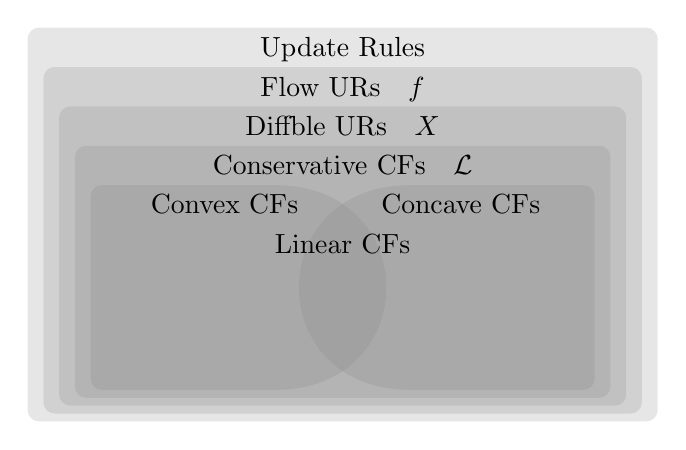
\begin{tikzpicture}
		\begin{scope}[fill=gray,fill opacity=0.2,rounded corners=4px]
			\fill (0,0) rectangle (8,5); % URs (Full Updates)
			\fill[] (0.2,0.1) rectangle (7.8,4.5); % Flow URs (Flows)
			\fill[] (0.4,0.2) rectangle (7.6,4.0); % Diffble URs (Vec Field)
			\fill[] (0.6,0.3) rectangle (7.4,3.5); % Conservative URs 
			\fill (0.8,0.4) -- (0.8, 3.0) -- (3, 3.0)
			 	to[out=0,in=0,looseness=2] (3,0.4) --cycle; % CONVEX
			\fill (7.2,0.4) -- (7.2, 3.0) -- (5, 3.0)
			 	to[out=180,in=180,looseness=2] (5,0.4) --cycle; % CONCAVE
		\end{scope}
		\begin{scope}[anchor=north]
			\node at (4.0, 5.0) {Update Rules};
			\node at (4.0, 4.5) {Flow URs~~~$f$};
			\node at (4.0, 4.0) {Diffble URs~~~$X$};
			% \node at (4.0, 3.5) {Conservative CFs~~~$\mathcal L$};
			\node at (4.0, 3.5) {Conservative CFs~~~$\mathcal L$};
			\node at (2.5, 3.0) {Convex CFs};
			\node at (4.0, 2.5) {Linear CFs};
			\node at (5.5, 3.0) {Concave CFs};
		\end{scope}
	\end{tikzpicture}
	\caption{%
		A map of different kinds of commitment functions and their representations.}
	\end{figure}
	}

\begin{figure*}
\centering
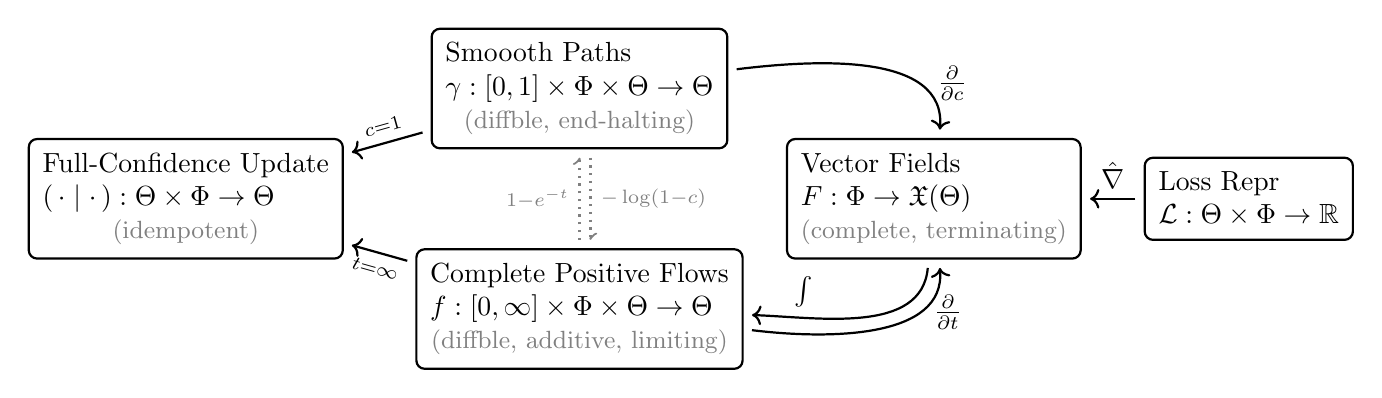
\begin{tikzpicture}
\begin{scope}[every node/.style={align=left,rounded corners=3,draw,thick,inner sep=5pt,anchor=center}]
	\node at (-5, 0) (fc) {Full-Confidence Update\\
		$(\,\cdot\mid \cdot\,) : \Theta \times \Phi \to \Theta$\\
			\small\hfill\color{gray}(idempotent)\hfill};
	\node at (0, -1.4)(flow) {Complete Positive Flows\\
		$f: [0,\infty] \times \Phi \times \Theta \to \Theta$\\
			\small\hfill\color{gray}(diffble, additive, limiting)\hfill};
	\node at (0, 1.4)(path) {Smoooth Paths\\ 
		$\gamma: [0,1] \times \Phi \times \Theta \to \Theta$\\
		\small\hfill\color{gray}(diffble, end-halting)\hfill};
	\node at (4.5, 0)(vfield) {Vector Fields \\
		$F : \Phi \to \mathfrak X(\Theta)$\\
		\small\hfill\color{gray}(complete, terminating)\hfill};
	\node at (8.5, 0) (loss) {Loss Repr \\
		$\mathcal L : \Theta \times \Phi \to \mathbb R$};
\end{scope}
	\draw[arr] (loss) to node[above]{$\hat\nabla$} (vfield);
%
	\draw[arr] (path) to[out=7,in=85] 
		node[right=5pt,pos=0.7]{$\frac{\partial}{\partial c}$} (vfield);
	\draw[arr] (flow) to[out=-7,in=-85]
		node[right=3pt,pos=0.7]{$\frac{\partial}{\partial t}$} (vfield);
%
	\draw[arr] (vfield) to[out=-95,in=-2] node[above=0pt,pos=0.75]
		% {$\int \mathrm dt$}
		% {$\int dt$} 
		{$\int$}
		(flow);
	% \draw[arr1] (vfield) to[out=90,in=0] node[below right]{$\int \mathrm dt$} (path);
	% \draw (vfield) to[out=90,in=0] node[above]{$\int \mathrm dt$} (flow);
	\draw[arr] (path) to node[above, sloped]{$\scriptstyle c=1$} (fc);
	\draw[arr] (flow) to node[below,sloped]{$\scriptstyle t=\infty$}(fc);
	
	\draw[arr,-left to,dotted,gray] (path) edge[transform canvas={xshift=4pt}] 
		node[right]{$\scriptstyle-\log(1-c)$} (flow);
	\draw[arr,-left to,dotted,gray] (flow) edge
	 	node[left]{$\scriptstyle1-e^{-t}$}(path);
	% \draw[arr,-left to] (path.south)++(0.1,0) to (flow.north)+(0.1,0);
	% \draw[arr,-left to] (flow.north) to (path.south);
\end{tikzpicture}
\caption{Different representations of update functions, and the relationships they have with one another. 
Sections 3 and }\label{fig:map}
\end{figure*}


\begin{example}\label{ex:jugo}
Jugo is an impartial juror.
Like the other jurors, she has two buttons in front of her.
The button labeled $\mathsf G$ increases the probability 
of a guilty verdict, while the button labeled $\mathsf N$ increases
the probability of a not-guilty verdict. 
In more detail: let $J$ be the number of jurors, and $G_j(t)$ be
a variable that is equal to one if juror $j \in \{0, \ldots, J\}$
is pressing the $\mathsf G$ button at time $t$, and zero otherwise; 
symmetrically, let $N_j(t)$ indicate whether $j$ is pressing the $\mathsf N$ at 
time $t$. The belief state of this automated system is
represented by a single number $g \in [0,1]$.
If any individual juror presses the $\mathsf G$ button, 
the system evoves according to $\frac{\mathrm dg}{\mathrm dt} = (1-g)$;
we call this the \emph{vector field} associated with the $\mathsf G$ button.
The total effect of all buttons is then the sum of that of all buttons across all vector fields, when they are active:
% in which case $g(t) = 1 + (g(0) - 1)e^{-t} $.
% Concretely, their dynamics are governed by:
\[
	\frac{\mathrm dg}{\mathrm dt} = 
	\sum_{j = 1}^J G_j(t) (1-g) 
		- g N_j(t)~,
	% \begin{cases}
	% 	(1 - p)	& \text{button $\uparrow$ pressed} \\
	% 	-p & \text{button $\downarrow$ pressed}
	% \end{cases}	
\]
so that $g$ exponentially approahces $1$ when more $\mathsf G$ buttons are pressed than $\mathsf N$ buttons,
and symmetricaly, exponentially approaches $0$ when more $\mathsf N$ buttons than $\mathsf G$ buttons are pressed.
At the end of the trial, the defendant is convicted with probability
equal to the final value of $g$. 

Let $\phi$ represent a piece of evidence suggesting guilt, presented by the
prosecution from time $t_1$ to time $t_2$,
and suppose for now that only buttons labeled $\mathsf G$ are pressed
in this interval.
% Many aspects of this scenario can be understood in terms of confidence.
%
	% The amount of time that 
	% What is the confidence of the system in that evidence, as it understands it from the Jurors?
% First, suppose that only $\mathsf G$ buttons are pressed
	 % between $t_1$ and $t_2$. 
% in between times $t_1$ and $t_2$.
The system measures $j$'s confidence in $\phi$ by
\[
	w_j := \!\int_{t_1}^{t_2}\!\! G_j(t) \mathrm d t 
	= \text{ total time $j$ presses $\mathsf G$ during $\phi$,}
\]
Note that $w_j = 0$ if and only if $j$ does not press any buttons,
which (a) indicates that $j$ does not trust the evidence $\phi$, 
and (b) communicates this fact to the system, by telling it to ignore 
the evidence. 
Note that this is an additive representation of confidence, since
pressing the button for four seconds, and then three more later, is
by definition the same as pressing it for seven. 
While the maximum possible confidence of $w_j$ is $(t_2 - t_1)$,
this system does not allow a juror to express \emph{full} confidence in $\phi$
because no finite amount of $\mathsf G$-pressing will result in a 
guilty verdict with probability one; it is always possible to increase
the value of $g$ through additional evidence. 

% Now, recall that ,
Altogether, the system's confidence in $\phi$ can be measured by
as the unique value $W$ for which
\begin{align*}
	% \int_{t_1}^{t_2} W (1-g(t)) \mathrm d t = \int_{t_1}^{t_2} \sum_{j=1}^J G_j(t) (1-g(t)) \mathrm d t,
	\int_{t_1}^{t_2} W (1-g(t)) \mathrm d t =
	 g(t_2) - g(t_1),
	% \\
	% W = \frac{1}{t_2-t_1 - \int_{t_1}^{t_2}g(t) \mathrm dt} \int_{t_1}^{t_2} \sum_{j=1}^J G_j(t) (1-g(t)) \mathrm d t
\end{align*}
which, so long as only $\mathsf G$ buttons are pressed, equals
$W := \sum_{j} w_j$, so this measure of confidence is additive 
across jurors as well as across time. 
This is appropriate, since the jurors are independent and 
not communicating with each other.
% This is a weighted sum of $w_i's$
As before, $W = 0$ if and only if no juror presses any buttons between times $t_1$ and $t_2$,
indicating zero trust leant to $\phi$. In such a case, the system ignores $\phi$ in updating its beliefs.
And just as no individual juror can send a full-confidence update to the system,
	the system cannot recieve a full-confidence from the jurors as a whole.
	
The picture gets significantly more complicated if we consider the possibility
that jurors might press the $\mathsf N$ button. For example, if $\phi$, which was intended
as evidence of guilt, has the effect of getting jurors to press $\mathsf N$, there is a sense
in which they have \emph{negative} confidence in $\phi$, since the belief update happened in the opposite direction of what $\phi$ represents; rather than \emph{no} trust, this is represents \emph{distrust}. 
Small negative updates are always possible except at the boundary of belief space, but in this paper, we focus almost entirely on positive confidence updates.

The introduction of the second button also uncovers a significant source of complexity:
unlike \cref{ex:prob-simple,ex:classifier,ex:shafer}, 
the order that evidence is presented matters, when there is more than one possible response to it.
Evidence presented later has a larger effect,
meaning that this system exhibits a recency bias.
% (This lack of commutativity corresponds to possibility that,
%	as a Lie algebra, the bracket may not be identically zero.)

Now consider a variant of this system that does
not trust all jurors equally; rather, it trusts each juror $j$
to a degree $\beta_j \in [0, \infty]$, and now $g$ evolves
according to
\[
	\frac{\mathrm dg}{\mathrm dt} = 
	\sum_{j = 1}^J \beta_j \Big( G_j(t) (1-g) 
		- g N_j(t) \Big).
	% \begin{cases}
	% 	(1 - p)	& \text{button $\uparrow$ pressed} \\
	% 	-p & \text{button $\downarrow$ pressed}
	% \end{cases}	
\]
In this case, the system can be said to have trust $\beta_j$ in juror
$j$, since $j$'s buttons are ignored when $\beta_j = 0$. 
When $\beta_j = \infty$ (an expression of full confidence in $j$),
$g$ immediately jumps to 0 when $j$ presses 
$\mathsf N$, or to 1 if $j$ presses $\mathsf G$ (unless canceled by
another full-confidence juror pressing the opposite button).
If all jurors have full confidence, then the verdict of this system is
a majority vote at the last moment a button was pressed. 
Thus, the weights attached to weighted combinations are (additive) expressions 
of confidence as well. 
\end{example}

\cref{ex:jugo} illustrates how a (sufficiently nice) vector field, 
	which is simpler than a smooth path for every starting point, is enough to define
an additive notion of confidence, via its integral curves.
It may seem strange to define confidence via a vector field, which does not mention confidence at all---but in a sense, it works because a vector field captures precisely everything about the update \emph{except} for the confidence. We do this formally in \cref{sec:vecrep}. 

In \cref{sec:loss-repr}, we demonstrate that it is typically possible to get an even more compact representation of the updating process, by representing the vector field implicitly as gradients of some ``loss function''.
To do this at full generality, we need to make sense of a gradient, which requires more structure, in the form of a Riemannian metric.  It turns out that, up to a multiplicative constant, there is a unique natural Riemannian metric on any parameterization of a probability distributions \cite{chentsov}; taking gradients with respect to this geometry, show how familiar loss functions on probability measures correspond to different standard notions of confidence in the other representations.

Once we have the formalism, fully in place, we give further examples of how confidence works in exponential families, in particular showing how Kallman gain and inverse variance can be viewed as confidence as well.
% Say 


\commentout{
This general idea can be cleaned up by appeal to differential geometry.
Fix an input $\phi$.
Assuming that the update paths are differentiable in the degree of confidence at any initial beleifs, the collection of updates with infinitessimal confidence forms a complete vector field $X_\phi$ over the space of beliefs, whose integral curves are paths in belief space, parameterized by confidence $\beta \in [0,\infty]$.
% Of course, we may always convert this number back to $[0,1]$,
We step through this more carefully in \cref{sec:field-repr}.

%joe1*: NO!  This is not the place to bring up Reimannian metrics!
Finally, if our belief space is endowed with a Riemannian metric, so that we may take gradients, partial update functions may be specified by a loss.}


% natural measure of confidence that works in all cases,
% which 
% It turns out that there is a natural way of measuring confidence in all cases of interest, based on differential geometry of belief space. 
% Furthermore, in the case where belief states are Dempster-Shafer belief functions, 
% and inputs are simple support functions, this measure of confidence is what Shafer calls the ``weight of evidence''.
%% TODO: Shafer



% It is not always most natural for confidence to range between zero and one. 
% But there are many instances in which 
% However, there is a more universal representation of it in $[0, \infty]$

% While probability ranges from untenable (0) to undeniable (1),
% confidence ranges from completely untrustworthy $(\bot)$ to fully trusted ($\top$).




\commentout{
	\subsection{Other Conceptions of Confidence.}

	\textbf{Probability.}
	% Probability is a numerical scale that ranges from untenable (0) to undeniable (1).
	% No number on this scale is truly neutral.
	% One of the biggest shortcomings of probability is its inability to represent a truly neutral attitude towards a proposition.
	Some people do use ``confidence'' to mean the same thing as probability. When they say they have low confidence in $\phi$, they mean that they think $\phi$ is unlikely.

	One of the biggest shortcomings of probability is its inability to represent a truly neutral attitude towards a proposition.
	%  probability of $\frac12$ .
	% This shortcoming has perhaps been the primary selling point of many alternatives to probabiltiy, such as Dempster-Shafer Belief functions.
	A value of $\frac12$ may be equally far from zero as it is from one, but is by no means a neutral assessment in all cases: hearing that your favored candidate has a 50\% chance of winning is big news if a win was previously thought to be inevitable.
	For this reason, telling someone the odds are 50/50 is quite different from saying you have no idea.
	% By contrast, zero confidence represents a truly neutral stance; a statement with zero confidence has no effect.
	By contrast, zero confidence represents something truly neutral:
		a statement made with zero confidence does not stake out a claim, and
		a statement recieved with zero confidence does not affect the recipient's beliefs.
	Nevertheless, in some contexts, we will see that confidences correspond to to probabilities.

	\textit{Opacity.} To use a graphical metaphor, think of certainty as black or white.
	Probability describes shades of gray, while confidence describes opacity.
	If we are painting with black and start with a white canvas, there is a precise correspondence between the opacity and the resulting shade of gray.

	\textbf{Upper and Lower Probabilities.}
	Upper and lower probabilities can describe a neutral attitude towards a proposition, but they are not really a specification of trust, but rather a direct specification of a belief state.
	It isn't immediately clear how to use these representations of uncertainty to update, and they're a little too complex to function effectively as the primitive measure of trust that we're after.


	\textbf{Shafer's Weight of Evidence.}
	Shafer's ``weight of evidence'' is precisely the same concept we have in mind.
	Our analysis precsely reduces to his, in the setting where belief states are Belief functions (which generalize probabilities, but not, say, neural network weights), and observations are events.
	% This paper can be a generalization of Shafer's ``weight of evidence'' to a broader class of settings, where one might have very different belief states and observations.
	Thus, this paper can be viewed as generalizing this concept to a broader class of settings, without requiring that one adopt Shafer's conception of a belief state or an observation.


	\textbf{Variance and Entropy.}
	The inverse of variance, sometimes known as precision,
		is also commonly used to measure confidence.
	If a sensor is unreliable and can give a range of answers, the variance of the estimate is a very common way of quantifying this reliablility.
	If measurements have zero variance, in some sense one has absolute confidence ($\top$) in the sensor. If measurements have infinite variance, then in some sense one has no confidence in the sensor, since individual samples convey no information about the true value of the quantity measured.
	As with probability, inverse variance will coincide with confidence in some settings; we will see how in \cref{sec:variance}.

	Entropy, like variance, is a standard way of measuring uncertainty, and in some settings, confidence coincides with entropy (see \cref{sec:entropy}).
	The assumption underlying both approaches is that there's some ``true'' value of the variable, and that the randomness is epsistemic (due to sensor errors) rather than aleotoric (inherrent in the quantity being measured).

	\textbf{Confidence Intervals and Error Bars.}
	Another notion of the word ``confidence'' comes from the term ``confidence interval''.
	This concept arises in settings involving a probability distribution $\Pr(X)$ over a metric space $X$, typically $X = \mathbb R$.
	A 95\% confidence interval is the (largest) ball containing 95\% of the probability, and its size is a geometric measurement of how .
	This intuition behind this reading of the word confidence is the same as
}


\section{A Formalism For Updating}

Throughout, we use $\Theta$ to refer to some space of possible belief states,
and $\Phi$ for a set of possible inputs. 
\commentout{% have now already given these examples more clearly; now cut to the chase!
	For example, a belief state $\theta \in \Theta$
	might be probability distribution,
	a Dempster-Shafer belief function, or
	weights for a neural network,
	while an input $\phi \in \Phi$ might be an event, or a sample from a dataset. 
}
%
% $\Theta$ might be \textellipsis
% \begin{itemize}[nosep]
%     \item $\Delta W$, the set of probability distributions over measurable space $W$ of outcomes;
%     \item the set of parameters to some parametric family of distributions;
%     \item the set of belief functions over a common space of outcomes;
%     \item the set of all possible PDGs;
%     \item a set of worlds an agent considers possible;
%     \item
% % \end{itemize}
Now, suppose we have some initial belief state $\theta$, and observe $\phi$ with confidence $\alpha \in [0,1]$. 
How do our beliefs change as a result? 
To study this mathematically, we assume that the process can be captured in functional form:
\unskip\footnote{%
	% we can just as easily handle randomized updates;
	It should be straightforward to extend our theory
	so as to handle randomized updates as well;
	the point is that
	% the update can be prescribed by an algorithm.
	the belief state, observation, and confidence must together contain
	enough information to describe the updating process.
	}
\begin{CFaxioms}
	\setcounter{CFaxiomsi}{-1}
	\item
	% \item[CF0]
	There exists some function
	$
	% \[
		% F : \confdom \to ( \Phi \to ( \Theta \to \Theta) )
		F :  \Phi \times [0,1] \times \Theta \to \Theta
	% \]
	$
	which, given input $\phi \in \Phi$, confidence $\chi \in [0,1]$, and a prior belief state $\theta \in \Theta$, 
	produces the appropriate posterior belief state $F(\phi, \chi, \theta) \in \Theta$. 
	 % belief state $F^c_\phi\theta$ that corresponds to the result of observing $\phi$ in state $\theta$. 
	 	\label[CFaxiomsi]{ax:funcform}
\end{CFaxioms}

Given such a function $F$, as well as a statement $\phi \in \Phi$
and confidnece $\chi \in [0,1]$, we call 
$F^\chi_\phi = F(\phi, \chi, -) : \Theta \to \Theta$
% a (confidence-$\chi$) \emph{update}.
an \emph{update}.
To ensure $F$ captures the belief updating process, we also require that it satisfy some axioms, characterizing the important shared features between \cref{ex:prob-simple,ex:classifier,ex:shafer}.
First, we would like no-confidence updates to leave our belief state unchanged. 

\begin{CFaxioms}
	% \item \textbf{(zero)} $F^{0}_A(\Pr) = (\Pr)$
	% \item  $F^{0}_A  = {1}_{\Delta\X}$. (That is, $F^{0}_A(\Pr) = \Pr$ for all $\Pr \in \Delta\X$.)
	% \item  $F^{0}_\phi  = {1}_{\Delta\X}$. (That is, $F^{0}_\phi(\Pr) = \Pr$ for all $\Pr \in \Delta\X$.)
	%     \hfill \textbf{(zero)} \label{ax:zero}
	\item
		% $F^{\bot}_\phi  = {\mathrm{Id}}_{\Theta}$.\\
		% (That is, $F^{\bot}_\phi(\theta) = \theta$ for all $\theta \in \Theta$.)
		% For all $\theta \in \Theta$ and $\phi \in \Phi$, $F^{\bot}_\phi(\theta) = \theta$.
		% No-confidence updates are identities. 
		% That is,
		For all $\theta \in \Theta$ and $\phi \in \Phi$,
		 $F^{0}_\phi(\theta) = \theta$.
		% \hfill \textbf{(no-confidence)} 
		% \hfill \textbf{(no-conf)} 
		% \hfill \textbf{(zero)} 
		% \hfill \textbf{(neutrality)} 
		\label{ax:zero}
\end{CFaxioms}


% Thus, a no-confidence update simply discares the new observation.
% At the opposite extreme, we call $F^1_\phi$ a \emph{full update}. 
% The appropriate way to deal with full confidence depends
% At the opposite extreme, the appropriate way to deal with full confidence
The appropriate way to deal with full confidence, on the other hand,
depends on the relationship between $\Theta$ and $\Phi$,
but it still characterized by an important property.
% , but it can still be characterized at this level of generality.


% \textbf{High Confidence Updates.}
\subsection{Updating with Full Confidence}
Since the purpose of $F^1_\phi$ is to \emph{fully} incorporate $\phi$ into our beliefs,
two successive updates with the same information ought to have the same effect as a single one.
Intuitively, this is because if we have just updated our beliefs to be consistent with the information $\phi$, then a second observation of $\phi$ will require no further alterations of our belief state.
% In this case, we call $F$ an \emph{update rule}, or more precisely, a \emph{$\Theta$-update rule on $\Phi$}, and insist that

\begin{defn}
	A \emph{full-confidence ($\Theta$-)update rule} (for $\Phi$) is
	a mapping $P: \Phi \times \Theta \to \Theta$ such that
	for all $\phi \in \Phi$, 
	$P_\phi = (\theta \mapsto P(\phi,\theta)): \Theta \to \Theta$ is idempotent.
	That is,	
	$P_\phi(P_\phi(\theta)) = P_\phi(\theta)$
	 for all $\phi\in\Phi$ and $\theta \in \Theta$.
\end{defn}

\begin{CFaxioms}
	\item
	% Full-confidence updates are idempotent.
	% For all $\phi \in \Phi$, the update $F_\phi$ is idempotent.
    % That is, for all $\phi \in \Phi$,  $F^1_\phi \circ F^1_\phi = F^1_\phi$.
    % That is, for all $\phi \in \Phi$ and $\theta \in \Theta$,  $F^1_\phi \circ F^1_\phi = F^1_\phi$.
    % (i.e., $F^1_\phi \circ F^1_\phi = F_\phi$).
	Full-confidence updates are idempotent. Or,
	equivalently,
	$F^1 = (\phi, \theta) \mapsto F(\phi,1,\theta): \Phi \times \Theta \to \Theta$ is a full-confidence
	update rule.
	\label{ax:idemp}
\end{CFaxioms}



% In curried form, $F : \Phi \to (\Theta \to \Theta)$.

% We now proceed with the formal details.
% \textbf{Update Rules.}
% Consider a space $\Theta$
% of possible belief states,
% and a set $\Phi$ of statements.
% % and a set $\Phi$ of ``statements'', i.e., the things one can have confidence in.
% % An \emph{update rule} (or more precisely, a \emph{$\Theta$-updating rule on $\Phi$})
% An \emph{update rule}, or more precisely, a \emph{$\Theta$-update rule on $\Phi$},
% is a function of the form
% \[
%     % F :  (\mathbb R \times \Phi) \to \Big( \Theta \to \Theta \Big)
%     F :  \Phi \to \Big( \Theta \to \Theta \Big)
% \]
% % which describes how to update beliefs about $X$, with the new information, at a certain level of trust.
% which describes how to (fully) update beliefs $\Theta$ with new information $\Phi$.
% and for $F$ to be an update rule, we require that , meaning that updating any belief with $\phi$ twice in a row is equivalent to single update.
% Having said that, one reading of this paper is a relaxation of this requirement.
% Here are some examples.
Once $\Theta$, $\Phi$, and any implicit structure in them is specified, there is often a natural choice of full-confidence update rule.
To illustrate, we now consider three different rules for different choices of $\Phi$.
In each case, the possible belief states $\Theta := \Delta W$ be the set of all probability distributions over a finie set $W = \{w_1, \ldots, w_n\}$ of ``possible worlds''.

\begin{enumerate}[wide, label=\textbf{\thesubsection.\arabic*}]
	\item %\textbf{Conditioning.}
	\textbf{Conditioning.}
	First, consider the case where observations are events, i.e., $\Phi := 2^W$.
	% One particularly natural $\Delta W$-update rule on $2^W$ is given by conditioning,
	% Here, the appropriate update seems to be condition:
	Here, the appropriate rule seems to be conditioning:
	% \[
	% \begin{aligned}
	% 	(-) \smash{\,\Big|\,} (\;\cdot\;) : \qquad 2^W &\to (\Delta W \to \Delta W) \\
	% 	A  &\mapsto (  ~\mu~~ \mapsto \mu \mid A ~),
	% \end{aligned}
	% \]
	% where $(\mu \mid A)(x) = \frac{\mu(\{x\})}{\mu(A)}$
	% in which learning $A$ maps
	% where the action of the conditional measure $\mu\mid A$ is given by $(\mu \mid A) \{w\} = \ifrac{\mu\{w\}}{\mu(A)}$.
	% where the action of the conditional measure $\mu\mid A$ is given by $(\mu \mid A)(B) = \ifrac{\mu(B \cap A)}{\mu(A)}$, provided $\mu(A) > 0$,
	starting with $\mu \in \Delta W$, the conditional measure 
	$\mu\mid A$ is given by $(\mu \mid A)(B) = \ifrac{\mu(B \cap A)}{\mu(A)}$, provided $\mu(A) > 0$,
	% and may be defined arbitrarily otherwise.
	and otherwise is just equal to $\mu$.
	Observe:
	\begin{itemize}[nosep, leftmargin=1.2em]
		\item Provided $\mu(A) > 0$, then $(\mu\mid A) \mid A = \mu \mid A$, so conditioning is a full-confidence update.
		\item If $\mu(A \cap B) > 0$, then $(\mu \mid A) \mid B = \mu \mid (A \cap B) = (\mu \mid B) \mid A$, so the order that information is recieved does not matter (so long as it is consistent with one's beliefs).
	\end{itemize}
	There are well-known issues with conditioning $\mu$ on $A$ when
	$\mu(A) = 0$, typically this operation is undefined. Note that to satisfy
	\cref{ax:idemp}, the result must either be $\mu$ itself or a
	 distribution that gives probability 1 to $A$. 
	% However, it is not the only $\Delta W$-updating rule for $2^W$.
	 % $\Phi$.

	\item
	\textbf{Imaging.}
	A second example of an update rule is the ``imaging'' approach of David Lewis
	\parencite{lewis1976probabilities}.
	% , albeit in very different notation.
	% Once again, consider a finite set $W$, and belief states $\Theta := \Delta W$.
	Suppose that, for some set $\Phi$, that we already have a full-confidence update rule
	$f : \Phi \times W \to W$ on individual worlds, which we interperet as assigning each statement $\phi \in \Phi$ and $w \in W$ an element $f(\phi, w) \in W$ which is the unique ``world most similar to $w$, in which $\phi$ is true'' \parencite{gardenfors1979imaging}.
	In this case, idempotence of $f_\phi: W \to W$ amounts to the (very reasonable) requirement that the world most similar to $f_\phi w$ in which $\phi$ is true, is $f_\phi w$ itself.
	From $f$, we can construct a full confidence update rule $F$ for $\Delta W$
	with the pushforward	
	\[
    	\begin{aligned}
    		% F_\phi(\mu) &:=
    		F(\phi, \mu) 
				% &:=
				% f^{\sharp}(\mu)
    			% &= A \mapsto \mu( f^{-1}_\phi( A ))\\
    			&= A \mapsto \mu(\{w : f(w, \phi) \in A\})
    	\end{aligned}
		% \qquad
		% \qquad
		% \begin{tikzpicture}[center base]
		% 	\node[dpad0] (W) {$W$};
		% 	\node[dpad0, right=1 of W] (W') {$W$};
		% 	\node[dpad0, below right=0.2 and 0.2 of W] (Phi) {$\Phi$};
		% 	\mergearr{W}{Phi}{W'}
		% 	\node[above=1pt of center-WPhiW']{$f$};
		% 	\draw[arr2, <-] (W) to node[above]{$\mu$} ++(-1, 0);
		% 	\draw[arr2, <<-] (Phi) to node[below]{$\phi$} ++(-1.3, 0);
		% 	\draw[arr2, <-, dashed, gray] (W') to node[above]{$F_\phi(\mu)$} ++(2, 0);
		% \end{tikzpicture}
	\]
	which intuitively moves the probability mass on each world $w$ to the $f_\phi w$, the closest world to $w$ in which $\phi$ is true.
	% is the pushforward measure of $\mu$ through $f_\phi$, which Lewis calls the ``image of $\mu$ on $\phi$''
	And, since $f$ is idempotent, $F$ will be as well.


	\commentout{
	\item More generally, consider a measurable space $\mathcal W = (W, \mathcal A)$, where $W$ is a set and $\mathcal A$ is a $\sigma$-algebra over $W$, and let $\mathcal F \subset \mathcal A$ be closed under supersets in $\mathcal A$.
	% Now, let $\Theta$ be the set of conditional probabili$

	\TODO[Properly Use Conditional Probability Measure, to define on all events]

	Conditioning a probability distribution $\mu \in \Delta\X$ on an event $A \in \mathcal A$ also makes sense in this more general measure-theoretic setting, at least so long as $\mu(A) > 0$, and is given by
	% the Lebesgue integral
	% \[
	$$
		% (\mu \mid A) (B) = \frac{1}{\mu(A)} \int \mathbf 1_{B}(x)  \mathrm d\mu(x)
		(\mu \mid A) (B) = \frac{\mu(B \cap A)}{\mu(A)}
	$$
	}


	\item
	\textbf{Jeffrey's Rule.}
	% Once more, suppose that $W$ is a finite set and $\Theta := \Delta W$.
	Next, consider a more general form of observation, in which observations themselves are probabilities.
	% Formally, suppose $\Phi$ consists of pairs $(X,\pi)$,
	Formally, let $\Phi$ be the set of pairs $(X,\pi)$,
	% Formally, suppose $\Phi$ consists of marginal distributions $\pi(X)$
	% Formally, suppose $\Phi$ consists of distributions $\pi(X)$,
	% written $\pi(X)$,
	where $X : W \to S$ is a random variable taking values in some set $S$,
	% (i.e., some function of $W$),
	and $\pi \in \Delta S$ is a probability on
	% the possible values that $X$ can take.
	$S$.
	Jeffrey's rule is then:
	\begin{align*}
		% \mathrm{Jeffrey}_{(X,\pi)}
		% \mathrm{Jeffrey}_{\pi(X)}
		% \mathrm{J}_{\pi(\mskip-2muX\mskip-2mu)}
		\mathrm{J}_{(X,\pi)}
		(\mu) &:= \sum_{x \in S} \pi(X{=}x) \;  \mu \big|
            (X{=}x)
            % \{ w : X(w) = x \}
			% \\
			% &= A \mapsto \sum_{x \in S} \pi(X{=}x)\, \mu( A \mid X \!= x)
	\end{align*}

	When $\pi$ places all mass on some $x \in S$, Jeffrey's Rule amounts to conditioning on $X {=} x$.
	 % but for other choices of $\pi(X)$,
	For this reason, Jeffrey's Rule is sometimes often thought of as a generalization of conditioning that admits for less that complete certainty.
	However, it is still a full-confidence update rule---just one that handles observations that can be uncertain.

	Let $\mu' := J_{\pi(X)}(\mu)$ be the result of applying Jeffrey's rule for $(X,\pi)$ to $\mu$.
	% then $\pi$ will be fully incorporated (that is, $\mu'(X) = \pi(X)$),
	Note that $\mu'(X) = \pi(X)$, so $\pi(X)$ has been fully incorporated into $\mu'$, while all information about the old prior belief about $X$ has been destroyed by the update.
\end{enumerate}


\subsection{%
	% Continuity and
 	The Path of Middling Confidence}

Full updates are quite extreme.
An agent that updates by conditioning, for instance,
% is permanently commited to believing everything it ever learns with perfect certainty,
permanently commits to believing everything it ever learns,
and gains nothing from making the same observation twice.
 % (\cref{ax:idemp})
% Humans don't work this way. The effectiveness of flash cards as a learning tool demonstrates this clearly: if we were using an update rule, two cycles through a deck of flash cards would be no different from one.
Clearly humans are not like this; revisiting information
 	improves our learning \parencite{ausubel1965effect}.
Similarly, artificial neural networks are trained with
 	many incremental updates, and benefit from seeing 
	the training data many times.
% Indeed, this is one biggest differences between modern machine learning techniques and  older rule-based ones: modern algorithms update parameters little-by-little, rather than fully incorporating input information.
% Once an agent that uses conditioning incorporates $A$, it is forever committed to believing $A$, and as a side effect, there is no point to making
We would like an account that allows for for less extreme belief alterations,
in which information is only partially incorporated.
This is the role of intermediate values of confidence.

Since confidence is supposed to interpolate between prior beliefs and full update,
we would like each $\chi \mapsto F(\theta,\chi,\phi) : [0,1] \to \Theta$
to be a continuous path in belief states, from the initial belief to full incorporation.

\begin{CFaxioms}[nosep]
	\item
	$\Theta$ comes with a topology, with respect to which
	the restriction
	$F_{\phi}|_\theta : [0,1] \to \Theta$
	is continuous
		% for all $\phi, \theta \in \Phi\times\Theta$.
	for all $\phi \in \Phi$ and $\theta \in \Theta$.
	\label{ax:cont}
\end{CFaxioms}


% For this to be meaningful, we need $\Theta$ to be a topological space,
% in which case the simplest and most convenient thing would be to require:

It would be particularly nice if updates were continuous in our initial
beliefs as well: after all, similar priors typically result
in similar posteriors beliefs. This would allow us to strengthen
\cref{ax:cont} to something simpler:

\begin{CFaxioms}[nosep]
	\item
	% [TOP]
	% [CF{\the\numexpr\value{CFaxiomsi}+1\relax}${^\prime}$]
	[CF{\the\numexpr\value{CFaxiomsi}\relax}${^\prime}$]
	% $\Theta$ is a topological space, and
	$\Theta$ comes with a topology, with respect to which
	% \item
	$F_\phi : [0,1] \times \Theta \to \Theta$ is continuous
	for all $\phi \in \Phi$.
	\label{ax:cont-strong}
\end{CFaxioms}

Unfortunately, this is too strong to handle extreme beliefs.
In the probabilistic case, for instance:

% Axiom \cref{ax:cont-strong} says more---it says that the posterior 
% belief is also continuous in the prior beliefs, 
% which also seems appropriate. But this assumption has significant bite.

% \commentout{%
% actually, this shows a problem with defining 
%
% \begin{example}
% 	Again let $W$ be a finite set, and choose disjoint non-empty subsets
% 	$A, B \subset W$ with $A \cap B = \emptyset$.
% 	Let $p\ne q$ be two distinct distributions over $W$ supported
% 	on $A$, and $d$ be one suppoerted on $B$. Now, consider 
% 	% and consider a sequence $(\mu_i)_{i \in \mathbb N}$ of positive probability 
% 	% distributions over $W$ whose limit 
% 	% is the point mass $\delta_w$ on a particular world $w \in W$.
% 	% $\mu^*$ has support $A \subsetneq W$ (i.e., $\mu^*(A)=1$).
% 	the two sequences of probability distributions
% 	\[
% 		\Big(p_n= (1-e^{-n}) d + (e^{-n}) p \Big)_{n \in \mathbb N}
% 		,
% 		\qquad
% 		\Big(q_n = (1-e^{-n}) d + (e^{-n}) q \Big)_{n \in \mathbb N},
% 	\]
% 	both of which have limit $d$. But every $p_n | A = p$ while every $q_n |A = q$, so
% 	now \cref{ax:cont-strong} implies that 	
% \end{example}%
\begin{prop}
	There is no continuous extension of conditioning to a function
	$F$ satisfying \cref{ax:cont-strong}.
	% nor even one whose restriction to  $ [0,\epsilon) \times \Phi \times \Theta \to \Theta$
	% is continuous, for $\epsilon > 0$.
\end{prop}
% \begin{proof}
% 	Conditioning itself cannot even be extended to
% 	to a continuous (total) function $\Delta X \times 2^X \to \Delta X$,
% 	because there is no adequate way to handle probability-zero events.
% \end{proof}
% }%
This is a consequence of the fact that there's no way to extend
conditioning continuously to zero-probability events. 
What we can do is to define a set $\Theta_\phi$ of belief states that do not
outright contradict $\phi$, and ask that $F_\phi$ is continuous when 
restricted to this set. 
% It turns out that 
Better yet, we can do the reverse, and define $\Theta_\phi$ as the set
of beliefs on which $F_\phi$ is continuous.
% This can be done purely in terms of the continuity of $F$.

\begin{prop}
	There is a maximal open set $\Theta_\phi \subseteq \Theta$ such that
	 % and ask that $F_\phi$ is continuous on that set. 
	the restriction $F_{\phi} |_{\Theta_\phi} : [0,1) \times \Theta_\phi \to \Theta$
	is continuous. 	
\end{prop}
% \begin{defn}
 	% Given $\Theta$, $\Phi$, and $F$, d
% \end{defn} 

In \cref{ex:prob-simple}, $\Theta_\phi = \{ \mu \in \Delta W : \mu(\phi) > 0\}$.
In \cref{ex:classifier}, $\Theta_\phi$ consists of all weights $\mat w$ 
such that
the loss $\mathcal L(\mat w, \phi) < \infty$ that the training algorithm minimizes is finite.



% \textbf{Differentiability}.
% A primary goal of this paper is to study how updates are made in low-confidence settings.
% Confidence is meant to interpolate between fully incorporating information and ignoring it.
Confidence interpolates between ignoring and fully incorporating 
information. This interpolation becomes more useful
if it is not just continuous, but differentiable as well.
% After all, that was one of our motivations for focusing on confidence domains that can be represented as a real number.
% Next, we present two variants of a differentiability axiom, depending on the structure one has in hand. 

\begin{CFaxioms}
	\item \label{ax:diffble}
	$\Theta$
	carries a differentiable structure,
	\unskip\footnote{
		That is, either 
		$\Theta$ is either a subset of $\mathbb R^n$,
	 	or a differentiable manifold (with corners) 
		\parencite{lee2013smooth,joyce2009manifolds-w/corners}.}
	and for all $\phi \in \Phi$ and $\theta \in \Theta$, 
	the function $[0,1) \ni \chi \mapsto F(\theta,\chi,\phi) \in \Theta$
	is differentiable.
\end{CFaxioms}

To motivate our next axiom,
suppose that we learn $\phi$ with some small degree of confidence $\chi$,
but then immediately realize that we should have updated with higher confidence. 
To fix this, it seems clear that we need to gain additional confidence
in $\phi$, which can be done with a second update 
(with a smaller residual degree of confidence).

\begin{CFaxioms}
	\item 
	% More precisely, 
	% If $\chi_2 > \chi_1$, 
	% If $0 \le \chi_1 < \chi_2 < 1$, 
	If $0 < \chi_1 < \chi_2 < 1$, 
	then for all $\theta \in \Theta$, 
	there exists 
	% $\chi_{1{\to}2}^\theta \in [0,1]$
	% $\chi_{1{\to}2} \in [0,1]$
	% $\chi_3 \in [0,1]$
	% $\chi_3 \in [0,\chi_2]$
	$\chi_3 \in (0,\chi_2)$
	such that
	$
	F_\phi^{
	% \chi_{1{\to}2}^\theta
	% \chi_{1{\to}2}
	\chi_{3}
	}(F_\phi^{\chi_1}(\theta)) = F_\phi^{\chi_2}(\theta).
	$
	\label{ax:seq-for-more}
\end{CFaxioms}

The point of the monotonicity condition \cref{ax:seq-for-more} is to rule out cases such 
as the one depicted below, in which ``resuming'' an update
results in a totally different set of belief states.
\begin{center}
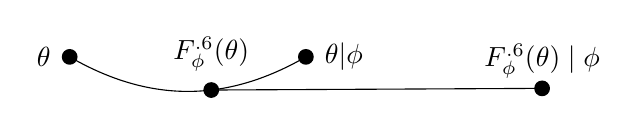
\begin{tikzpicture}
    \coordinate[label=left:$\theta~$] (A) at (0,0);
    \coordinate[label=right:$~\theta|\phi$] (C) at (3,0);
    \coordinate[label=above:$F_\phi^{.6}(\theta)\mid\phi$] (C') at (6,-0.4);
    \draw (A) to[bend right] 
		node[outer sep=0,pos=0.6,label=above:$F_\phi^{.6}(\theta)$](B){} (C);
    \fill 
        (A) circle (0.1)
        (B) circle (0.1)
        (C) circle (0.1)
        (C') circle (0.1);
    \draw (B.center) to (C');
\end{tikzpicture}
\end{center}
% \cref{ax:seq-for-more} also has a more significant effect: it means
\cref{ax:seq-for-more} also ensures
that a high confidence update can be decomposed into
several updates of lower confidence. 


Finally, we impose a mild regularity condition
that can be thought of as
% a special case arising in 
a limit \cref{ax:seq-for-more}
when confidences $\chi_1$ and $\chi_2$ become infinitessimally close;
% for infinitessimal values of confidence (specifically $\chi_1$),
% which we can make sense of because of \cref{ax:diffble}. 
% which we can make sense of via differentiability (\cref{ax:diffble}). 
we make this precise via differentiability (\cref{ax:diffble}). 
% The next axiom states
% This is a relatively minor condition

\begin{CFaxioms}
	\item \label{ax:nopause}
	If
	% $\frac{\partial}{\partial\chi} F(\theta,\chi,\phi) \!=\! 0$
	$\frac{\partial}{\partial\chi} F^\chi_\phi(\theta) = 0$
	and $\chi' > \chi$,
	then 
	% $F(\theta, \chi', \phi) \!=\! \theta$.	 
	$F^{\chi'}_\phi(\theta) = \theta$.	 
\end{CFaxioms}

Intuitively, \cref{ax:nopause} amounts to requiring that updates
do not ``temporarily pause'' for intermediate values of confidence,
and then resume for higher values of confidence.
The culmination of these axioms results in our first definition of an
update function that takes confidence into account.


% For this reason, we give them a special name
% Together, these axioms allow us to define an update rule, by:

\begin{defn}
	A function $F: \Phi \times [0,1] \times \Theta \to \Theta$ 
	satisfying
	\cref{ax:zero,ax:idemp,ax:cont,ax:seq-for-more,ax:diffble,ax:nopause}
	is 
	% an \emph{update function}.
	a \emph{path update function}.
\end{defn}



Path update functions capture some important aspects of uncertain
updating%
---but a number $\chi \in [0,1]$ is not the only useful
way to quantify confidence.
For the full picture of of how these concepts are related, we will
need to look at confidence from several more angles.

% If $\phi_1$ and $\phi_2$ are such that
% $F_{\phi_1}$ and $\phi_2$



% Intuitively,
% \cref{ax:seq-for-more} 
% says that 


\section{Fractional Updates, and the
    Flow Representations}


% , at a certain level of trust.
% We are interested in . A \emph{}
% Each of these update rules takes its
If we take a step back, fully incorporating information is really quite extreme.
% For agents that uses conditioning, for instance, incorporation is permanent.
% Observing information
An agent that updates with conditioning for instance, is forever committed to fully believing $A$, and consequently, learns nothing from observing $A$ agin in the future.
Humans don't work this way.
The effectiveness of flash cards as a learning tool demonstrates this clearly:
if we were using an update rule, two cycles through a deck of flash cards would be no different from one.
Similarly, artificial neural networks are trained with many incremental updates, and cycle through training data more than once.
Indeed, this is one biggest differences between modern machine learning algorithms and the older rule-based ones: the new ones update parameters little-by-little, rather than fully incorporating input information.
% Once an agent that uses conditioning incorporates $A$, it is forever committed to believing $A$, and as a side effect, there is no point to making
How shall we alter our picture to account for less extreme belief alterations, in which information is only partially incorporated?
This is where confidence comes in.
% This is where other value confidence comes in.
% Humans don't always update our beliefs with update functions.
% Often there seems to be value in learning the same thing more than once---or, put another way---in updating with confidence.


% To that end, we now consider a domain of possible values of confidence, which describes a degree of incorporation.
% To that end,


% We now define a \emph{\cofunc} to be a function

Let $\confdom$ be the set of possible confidences, which, for now, we will take to be the interval $[0, 1]$.
% We are now in a position to consider confidence when updating.
We are now in a position to take confidence into account in our updates.
As before, our first axiom is that we can capture the updating process in functional form.

\begin{CFaxioms}
	\item[CF0]
	There exists some function
	% $F : \Theta \times \Phi \to \Theta$,
	\[
		F : \confdom \to ( \Phi \to ( \Theta \to \Theta) )
	\]
	which, given a confidence and new information $\phi$, in addition to a prior belief state $\theta$, produces the belief state $F^c_\phi\theta$ that corresponds to the result of observing $\phi$ in state $\theta$. \label[CFaxiomsi]{ax:funcform}
\end{CFaxioms}

% Although not incontrovertable, this seems like a reasonable requirement.
% After all, if
% Although not incontrovertable, this seems like a reasonable requirement.
% It is not so important that the function be deterministic---we can make it a non-deterministic or probabilistic without too much hassle---the real purpose of \cref{ax:funcform} is to assert that all of the information we need to compute the next belief state is contained in either
% % (1) our previous belief state, (2) the new information, or (3) our confidence in it.
% in our prior belief state $(\theta)$, the new information $(\phi)$, or our attitude towards it ($c$).

Historically speaking, \cref{ax:funcform} has not proved as anodyne as it looks.
Some might object that it's not possible to write such a function that is appropriate in all circumstances.
For example, Shafer argues for Dempster's rule of combination as a way of incorporating information, but is very careful to emphasize that it ought to be used only on \emph{independent} information, for reasons illustrated below.



\begin{example}\label{ex:dupl}
	You have initial belief state $\theta_0$.
	Now, someone comes up to you and tells you that $\phi$ is true, a statement
		that you trust to some intermediate degree of confidence $c \notin\{ \bot, \top\}$.
	So, in accordance with \Cref{ax:funcform}, you use $F$ to transform your beliefs, partially incorporating the information to arrive at some belief state $\theta_1 := F^c_\phi(\theta_0)$.
	Immediately afterwards, your friend repeats what they just said: $\phi$ is true.
	Your confidence in the statement remains the same, and so according to
	\Cref{ax:funcform}, you again update your beliefs, arriving at $\theta_2 := F^c_\phi(\theta_1)$.
	Except in very special circumstances (e.g., you already know that $\phi$ is true, or $c \in \{\bot,\top\}$), typically $\theta_2$.
	And yet, it seems your your attitude towards $\phi$ ought to be the same whether you've heard it twice or only once.
\end{example}


Now, it's important to mention that we're not quite in the same position as Shafer.
Shafer was prescribing a concrete representation of $\Theta$ (a belief function) and a concrete update rule $F$ (Dempster's rule of combination), and so he needed to defend these choices.
% To take an analogous prescriptive stance,
We only need to defend something much more modest: we only need to defend the assumption that, if $\Theta$ and $\Phi$ properly model the relevant aspects of the scenario at hand, then there exists \emph{some} function $F$ which performs updates appropriately.
Descriptively speaking, we're also in good shape: for synthetic agents, it suffices to point out that learning algorithms represent functions, which given a state, an input, and a number of iterations (confidence), produce an output.
And, supposing that $\Theta$, $\Phi$, and $\confdom$ all capture the relevant respective aspects of a human's belief state, input information, and attitude towards it, how could it be that a human does otherwise?
%
% After all, if you recieve the same input twice, and your confidence in it has not changed, it would be best to only update once.
% There are essentially three ways to proceed.
In any case, keeping \cref{ex:dupl} in mind, here are three ways to proceed.

\begin{enumerate}[label={\textbf{I\arabic*.}},ref={I\arabic*}]
	\item \textbf{Accept Severe Limiations.} \label{approach:assume}
	Like Shafer, we could be careful
	% not to claim anything about how to update beliefs, except
	to claim nothing about the belief updating process except in the (unusual) case where
	information recieved is independent.
	% This severly handicaps the usefulness of .
	This would be a severe limiation to the theory, and much less necessary than it was for Shafer.
	Imagine that we are writing code that describes how a synthetic agent updates its beliefs. Shafer's approach is to package any such code with a warning against running it unless assured that observations will always be independent.
	But independece is notoriously difficult to establish; are we to simply accept that the code will not behave correctly in any realistic scenario?
	% Under what circumstances could we possibly be sure that all inputs we will be independent?

	In practice, many theoretical properties of standard statistical learning algorithms are heavily dependent on indepencence assumptions (most commonly, that one recieves independent, identically distributed samples).
	% Despite this, such algorithms .
	This warning label not seem to keep them from being applied in settings where practitioners readily admit samples are not really independent at all---nor indeed performing well emperically in those settings \parencite{???}.

	% If we need to make a decision that depends on information that is not given, then
	% Shafer found himself in a position where he needed to qualify usage of the update rule


	\item \textbf{Appropriately Enrich Domains.}\label{approach:enrich}
	% For instace, the agent has been totally
	% We told a story wanting to avoid incorporating information twice.
	In \cref{ex:dupl}, it seems obvious that we ought to ignore the second copy of the information, because it has already been accounted for.
	However, this intuition is highly contingent on the implicit supposition that we \emph{know} the second input to be a replica of the first.
	Were we ignorant to the nature of the second piece of information, perhaps it would not be so unreasonable to incroproate it again, even without a proof of independence.
	% If we want our agent to do the same
	% In asking our agent to take such issues into account, it is only fair to give it access to the same
	% It seems unfair to criticize an agent for not behaving
	So, if we would like our agent to make the same decisions that we did, it seems only fair to give it access to the knowledge that we needed to get there.
	One way of doing this is to extend the belief state so that it also tracks what information has been incorporated.
	% For instance, suppose that every message

	For \cref{ex:dupl} to work, it is critical that we are able to discern that the two inputs were identical.
	As a result, it seems that the relevant description of the input information was not just $\phi$, but a pair $(\phi, \mathit{id})$ that also a description of its identity.
	It is also critical that we remember the identity of previously incorporated information, so we would also be better off with a belief space $\Theta$ reflects this.
	With these two modifications, any \cofunc\ can be straightforwardly modified to avoid the issue in \Cref{ex:dupl}.


	We submit that it is always possible to enrich the space of beliefs and observations in this way to track the relevant information, to resolve the issue.
	With a few more assumptions later on, we will be able to formalize the construction we just alluded to (\cref{ex:dupl-enriched}).

	\item \textbf{An Incremental Interpretation of Confidence.}
		\label{approach:interperet}
	Finally, we can get around the issue by interpreting a confidence $c \in \confdom$ not as an absolute measurement of confidence, but rather an incremental one.  This means viewing $c \in \confdom$ as the degree of \emph{additional} confidence we have in $\phi$, beyond whatever we have already incorporated into our beliefs.

	% This proposal immediately raises some important questions.
	This proposal might be concerning.
	% First, how
	One might worry that it's harder to make sense of ``incremental confidence'' than an absolute notion.
	How ought we to numerically describe the confidence of an update?
	Suddenly this becomes much more subjective, for to assign a number, not only must we describe how much trust we have in the new information, but we must also take history or current belief state into account.
	Furthermore, the words ``incremental'' and ``additional'' suggest that we will need a formal description of how to aggregate confidences---%
	the very concept of which we will need to defend.
	% Indeed, such a way of combining confidences will ultimately play a large role for us.
	% It will turn out that such a way of combining confidences
	% Fortunately, it will turn out that

	Even modulo these concerns, the incremental interpretation still leaves us in a strictly better place than we were before.
	%  with \cref{approach:assume}.
	To begin, in situations where inputs are independent (i.e., the only cases where we would have been allowed to apply the \cofunc\ according to \cref{approach:assume}), the two notions coincide.
	More explicitly: if the new information $\phi$ is indepenendent of everything we've previously seen, then an absolute measurement of our confidence in it is no different from a measrurement of how much we ought to increment it from having no confidence.
	Already, though, we can do more.
	In the situation described by \cref{ex:dupl}, for instance,
	the second utterance induce no \emph{additional} confidence ($\bot$), and so applying $F$ with no confidence clearly gives the desired result of ignoring the new information (per \cref{ax:zero}).
%
%
	And even in general, the prospect of having to numerically estimate a fuzzy quantity seems more promising than red tape requiring that $F$ only be used (in good conscience) on independent information.
	% In some ways, this approach it is not so different from directly requiring independence of inputs, there are several aspects of this framing, that in our view, make it more pallatable.
	% First,
	% In cases
	% This raises some questions. Even if we already had a

\end{enumerate}


% We submit that any information that is relevant to that final belief state ought to be present in one of these places. For instance, if we've already heard this same information before, this fact should either be present in our beliefs $(\theta)$, in the observation $(\phi)$, or in the description of our confidence in it ($c$).


% which, given an incremental confidence $c \in \mathbb \confdom$, returns an ``incremental'' update rule, i.e., a function with the same type as an update rule, except possibly non-idempotent.
% which, given a confidence $c \in \mathbb \confdom$, returns an ``incremental'' update rule,
% i.e., a function with the same type as an update rule, except possibly not idempotent.
% i.e., a function $F^c : \Phi \to (\Theta \to \Theta)$ that may not be idempotent.
Given a confidence $c \in \confdom$ and a statement $\phi \in \Phi$, we write
 % Given a piece of information $\phi \in \Phi$, , we write
% $F^\beta_\phi : \Delta\X \to \Delta X$
$F^c_\phi : \Theta \to \Theta$
for the update prescribed by the \cofunc\ $F$.
% Furthermore, we will insist that \cofunc s .
Furthermore, we will insist that \cofunc s respect our interpretation of confidence at the two extremes.
% , especially the following two.
\begin{CFaxioms}
	% \item \textbf{(zero)} $F^{0}_A(\Pr) = (\Pr)$
	% \item  $F^{0}_A  = {1}_{\Delta\X}$. (That is, $F^{0}_A(\Pr) = \Pr$ for all $\Pr \in \Delta\X$.)
	% \item  $F^{0}_\phi  = {1}_{\Delta\X}$. (That is, $F^{0}_\phi(\Pr) = \Pr$ for all $\Pr \in \Delta\X$.)
	%     \hfill \textbf{(zero)} \label{ax:zero}
	\item
		% $F^{\bot}_\phi  = {\mathrm{Id}}_{\Theta}$.\\
		% (That is, $F^{\bot}_\phi(\theta) = \theta$ for all $\theta \in \Theta$.)
		For all $\theta \in \Theta$ and $\phi \in \Phi$, $F^{\bot}_\phi(\theta) = \theta$.
		% \hfill \textbf{(no confidence)} \label{ax:zero}
		% \hfill \textbf{(zero)} \label{ax:zero}
		\hfill \textbf{(neutrality)} \label{ax:zero}
	% \item $F^{\beta_1}_A \circ F^{\beta_2}_A = F^{\beta_1 + \beta_2}_A$
	% \item $F^{\top} : \Phi \to (\Theta \to \Theta)$ is an update rule, i.e.,
	%     the funciton $F^{\top}_\phi : \Theta \to \Theta$ is an idempotent.
	\item
		% For all $\phi$,
		For all $\phi$,
		% $F^\top_\phi$
		$F^\top_\phi : \Theta \to \Theta$
		is an idempotent update.\\
		Equivalently, $F^\top: \Phi \to (\Theta \to \Theta)$ is an update rule.
		% the funciton $F^{\top}_\phi : \Theta \to \Theta$ is an idempotent.
% If $F$ is a \cofunc, then by \cref{ax:idemp}, $F^{\top}$ is an update rule, and we call $F$ a ``refinement'' of the update rule $F^{\top}$.
		\hfill \textbf{(certainty)} \label{ax:idemp}\\
		We call $F$ a \emph{refinement} of the update rule $F^\top$.
% \end{CFaxioms}
% The next axiom,
% \begin{CFaxioms}
	% \item For all $\beta_1, \beta_2 \in \mathbb R_{\ge 0}$,~
	%
	% \item For all $c_1, c_2 \in \confdom$,~
	%     $F^{c_1}_\phi \circ F^{c_2}_\phi = F^{c_1 \oplus c_2}_\phi$
	%     % \hfill \textbf{(additivity)} \label{ax:additivity}
	%     \hfill \textbf{(combination)} \label{ax:additivity}
\end{CFaxioms}
\Cref{ax:zero} captures the intuition that we should ignore information in which we have no confidence, while \cref{ax:idemp} formalizes the intuition that a full-confidence updates act as we imagined.
At this point, we would like to point out that those who find \cref{ax:zero} reasonable have implicitly either accepted either \cref{approach:assume} or \cref{approach:interperet}.

\begin{example}
	Suppose you first hear $\phi$ from a partially trusted source, and incroproate it into your beliefs appropriately.
	Then, the same source sends you a second message, which is obviously spam.
	In an absolute sense, you now have no confidence ($\bot$) in anything this source tells you, including (in retrospect) both messages.
	It seems appropriate to excise $\phi$ from your belief state in response, rather than leaving your belief state unchanged, as \cref{ax:zero} would prescribe.

	Note that in this scenario, while it seems that we ultimately have no confidence in $\phi$, it does not seem to be the case that we have no incremental confidence in $\phi$.
	Rather, the incremental confidence seems to be the inverse of the original confidence.
\end{example}

From this point forward, we use the incremental interpretation of confidence, with the understanding that
all of our results also admit a more conservative reading, in which confidence is measured absolutely, and also all applications of the function $F$ are independent. 


% \Cref{ax:additivity} states that, for all $\theta$, the function $c \mapsto F^c_\phi\theta : \confdom \to \Theta$ is a group homomorphism.
 % a confidence of $\top$ indicates that we are fully incorporating information into our beliefs.




\begin{phaseout}
and so for most of this paper, we take $\confdom := \Rplus$ to be the group of extended nonnegative real numbers under addition.
With this choice of confidence domain, \cref{ax:additivity} begins to have more bite, although, as we will see, the effect is more to pin down a coherent system of measurement, and does not appear to restrict modeling expressivness.
%
%
% Below is a concrete representative example of a \cofunc\ with our standard confidence domain $\mathbb R_+$.


Here are some more abstract examples of \cofunc s, with confidence domain
$\confdom := \mathbb R_+$.
\begin{enumerate}
\item
Once again, suppose $W$ is a finite set,
$\Theta := \Delta W$, and $\Phi := 2^W$.
Here are two natural \cofunc s for this scenario, both of which are refinements of conditioning.
\begin{itemize}
	\item
	$\displaystyle
		(F1^c_A \mu)(B) = (1-e^{-c}) \mu(B|A) +  e^{-c} \mu(B)
	$
	\item
	$\displaystyle
		(F2^c_A \mu)(B) \propto \mu(B|A)^{(1-e^{-c})} \mu(B)^{e^{-c}}
	$
\end{itemize}
The first \cofunc, $F1$, linearly interpolates between the result of ignoring the information contained in the event $A$ (i.e., leaving the belief state $\mu$ unchanged) and conditioning on $A$.
By contrast, $F2$ does a similar interpolation, but multiplicatively.

\item
	% \textbf{Neural Networks Updates.}
	% \textbf{Machine Learning.}
Suppose that $\Theta$ is the set of possible parameter settings for a neural network, which aims to predict an element of $Y \subset \mathbb R^{m}$ given an in put from $X \in \mathbb R^{n}$.
So, for each $\theta \in \Theta$, we have a function $f_\theta : X \to Y$, and for fixed $x \in X$, the function $\theta \mapsto f_\theta(x) : \Theta$ is differentiable.

% $\{ f_\theta : X \to Y \}_{\theta \in \Theta}$;
% perhaps it is the set of possible weights of a neural network.


 % suppose $\Theta$ is a set of parameter settings ,

% WE DO NOT WANT TO TALK ABOUT DS FUNCTIONS HERE BECAUSE THEY ARE VARIABLE CONFIDENCE.
\item
Again consider a finite set $W$ and suppose $\Theta$ consists of all Dempster-Shafer belief functions
\end{enumerate}



% By currying we
% \begin{prop}
%
% \end{prop}



We are particularly interested in the setting where $\Theta$ parameterizes a family of probaility distributions.
To that end, suppose that $\X = (X, \mathcal A)$ be a measurable space, so that $X$ is a set and $\mathcal A$ be a $\sigma$-algebra over it, let $\Delta \X$ denote the set of probability measures over $\X$,
and keep in the back of our heads an indexed family
% $\{ p_\theta ( X_\theta ) : \theta \in \Theta\}$.
$
	\mathcal P =
	\{ p_\theta \in\Delta\X \mid \theta \in \Theta \}
$ of probability distributions.
% If we take
\end{phaseout}

% For instance, starting with a distribution $\mu_0 \in \Delta \X$, we can \emph{compose} updates.
%
% % \[
% %     \mu_0
% %         \xmapsto{\displaystyle F^{.3}_{\mathit{Height}=5'11''}} \mu_1
% %         \xmapsto{\displaystyle F^{.6}_{\Pr(Y=1|X=3)=0.4}} \mu_2
% %         \xmapsto{\displaystyle F^{2.1}_{K_i(\varphi)}} \mu_3.
% % \]


\section{Differentiable Updates, and their
    Vector Field Representation}


% Suppose that the space $\Theta$ is actually a differentiable manifold.
% In this case, we might want want $F$ to be compatible with the differentiable structure.
% \begin{CFaxioms}
%     \item $\Theta$ is a differentiable manifold.
%         For fixed $\theta$ and $\phi$, the function $\beta \mapsto F^{\beta}_\phi(\theta)$
%         is continuously differentiable.
%             \hfill \textbf{(differentiability)} \label{ax:diffble2}
% \end{CFaxioms}
% If $\Theta$ is a differentiable manifold and 

%joe3: bad story. Just say that you want additivity.
%oli3: bringing up text about additivity, and reduing stress on scale.
% Recall that the number of training iterations $n$ in \cref{ex:classifier}
% and Shafer's weight of evidence $w$ in \cref{ex:shafer}
% are measurements of confidence that do not lie in $[0,1]$, but
%  rather in $[0,\infty]$. 
Nearly all quantities used in science 
and everyday life
can be measured additively:
if you have six (feet/meters/galons/joules/people/votes/dollars), 
and then you find seven additional (distinct) ones, then you have thirteen altogether. 
We would like a measure of confidence that also works this way.
The number of training iterations $n$ in \cref{ex:classifier}
and Shafer's weight of evidence $w$ in \cref{ex:shafer}
are both additive examples of confidence.
Because they are additive,
% such values of confidence must be closed under addition,
% and hence include 
these confidences must be closed under addition, and hence
% are numbers in $[0,\infty]$, rather than $[0,1]$. 
all real numbers must be valid confidences.
% In this case, 
% In such cases,
% Thus, 
% we must instead use an analogous function of the form 
the appropriate analogue is a function
\begin{equation}
	F : \Phi \times [0, \infty] \times \Theta \to \Theta
	\label{eq:zero-inf-form}
\end{equation}
satisfying 
%oli3: can now remove hedging because of \top in axioms before:
% modified versions of
\cref{ax:zero,ax:idemp,ax:cont,ax:diffble,ax:seq-for-more,ax:nopause}
% identical except with $\infty$ in place of 1. 
%oli3: and here...
% that use $\infty$ in place of 1 for the upper limit of confidence. 
% We abuse terminology by stating that $F$ satisfies these axioms.
One reason to prefer this scale is that it 
allows us to represent degree of confidence in a way that combines additively. 

\begin{CFaxioms}
	\item For all
		% $\beta_1, \beta_2 \in \Rplus$,~
		% $\beta_1, \beta_2 \in [0,\infty]$,~
		$\chi_1, \chi_2 \in [0,\infty]$,~
		% $F^{c_1}_\phi \circ F^{c_2}_\phi = F^{c_1 \oplus c_2}_\phi$
		% $F^{\beta_1}_\phi \circ F^{\beta_2}_\phi = F^{\beta_1 + \beta_2}_\phi$.
		$F^{\chi_1}_\phi \circ F^{\chi_2}_\phi = F^{\chi_1 + \chi_2}_\phi$.
		% \hfill \textbf{(additivity)} \label{ax:additivity}
		% \hfill \textbf{(additivity)}
		\label{ax:additivity}
\end{CFaxioms}

% Recall that \cref{ax:seq-for-more} implies the behavior of updates is generated by low-confidence updates.
Recall how \cref{ax:seq-for-more} allows us to decompose high-confidence updates into sequences of low-confidence ones;
\cref{ax:additivity},
which implies \cref{ax:seq-for-more}, describes a particularly convenient
way that the decomposition might work. 

% In fact, there is a unique additive 
\begin{defn}
	% A function satisfying
	A \emph{flow update function}
	is a function
	$F : \Phi \times[0,\infty] \times \Theta\to \Theta$
	satisfying 
	%oli3: no more heding, part 3.
	% the appropriate analogues of
	% \cref{ax:zero,ax:idemp,ax:cont,ax:seq-for-more,ax:diffble}
	\cref{ax:zero,ax:idemp,ax:cont,ax:diffble}
	and \cref{ax:additivity}.
\end{defn}

To some,
% \cref{ax:additivity} might be pallatable already,
\cref{ax:additivity} might already be pallatable,
% but it looks like it might be an assumption that significantly restricts the expressiveness of our framework.
% but it also might look like it might significantly restrict the expressiveness .
but it is clearly a nontrivial assumption, and looks like it might severely restrict the expressiveness of our update formalism.
% This is not the case.
Fortunately, this is not the case.
While \cref{ax:additivity} does significantly pin down how confidence 
can be measured, it has no effect on what confidence can express.  
% More concretely, for every confidence function that does not satsify \cref{ax:additivity}, we can 


\begin{linked}{theorem}{add-reparam}
	If $F$ satisfies \cref{%
		ax:funcform,%
		ax:zero,ax:idemp,ax:cont,ax:seq-for-more,ax:diffble,ax:nopause},
	% then there is a unique 
	then
	\begin{enumerate}
		\item Up to a positive multiplicative factor, in its confidence
		argument, there is a unique additive representation
		$^+\!F$ of $F$. 
	\end{enumerate}
	
	up to multiplicative 
	
	flow update rule
	 $^+\!F$
	that behaves like $F$ for low confience updates
	(and is also additive: \cref{ax:additivity}). 
	%
	% Moreover,
	Furthermore, there exists a function 
	% $g$, increasing in $\chi$ such that,
	$g$ such that,
	for all $\theta,\phi,$ and $\chi$,
	\[
		F( \phi, 
		% g(\phi,\beta,\theta),
			\chi,
		 \theta )
		 =
		{^+}\!F(\phi,~ 
		% \beta,
		g(\phi,\chi,\theta),~
		 \theta).
	\]
\end{linked}
Thus, updates performed with $F$ are equivalent
to updates performed with ${^+}\!F$, except that
the degree of confidence needs to be translated appropriately (via $g$).


% Moreover, 

% Recall that \cref{ax:seq-for-more} impilies that the behavior of updates
% is generated by low-confidence updates; we saw a particularly nice
% way of doing that in \cref{ax:additivity},
% which has the feature that confidence behaves the same way no matter what your initial beliefs are. 


% Even restricting to , additivity is a particularly natural. 
% 
% \begin{prop}
% 	If $F$ is a differentiable \cofunc\ with confidence domain $\Rplus$,then there is a unique update rule $G$ with the same confidence domain, that behaves approximately like $F$ for small increments of confidence, and is also additive (\cref{ax:additivity}).
% \end{prop}


\subsection{Vector Field Representations}
\label{sec:vecrep}

We now turn to another representation of additive 
update functions, as vector fields. 
This representation allows us to extend the set $\Phi$ of possible observations to 
% to a set $\ext\Phi \supseteq \Phi$ with some algebraic operations.  
to a larger set $\ext\Phi \supseteq \Phi$ with some algebraic operations.  

In \cref{ax:diffble}, we assumed that $\Theta$ has a differentiable 
structure; thus, it makes sense to talk about its tangent space
%joe3: please add parens!
%oli3: parens are non-standard in this context. See Lee 2013,
%   which is the standard reference on manifolds, or even the 
%   wikipedia page. 
$T\Theta$,
which consists of pairs $(\theta, \mat v)$, where
$\theta \in \Theta$, and $\mat v$,
% is intuitively an infinitessial direction rooted at $\theta$.
intuitively, is a direction that one can travel in $\Theta$ beginning at $\theta$
% tangent to $\Theta$
% rooted at $\theta$
\parencite[\S3]{lee2013smooth}.
% structure; for ease of presentation, suppose that it is an $n$-dimensional manifold \parencite{lee2013smooth}. 
% For a smooth manifold $M$ (such as the space $\Delta \X$ of distributions over $\X$),
% and a point $p \in M$, we follow convention by writing $T_p M$ for the tangent space to $M$ at point $p$ \parencite{lee2013smooth}, and % $TM := \sqcup_{p \in M} (p, T_p M)$
% $TM := \sum_{p \in M} T_p M$ for the full tangent bundle over $M$.
%
% A vector field over $M$ is a smooth map $\mat v : M \to T M$ assigning a tangent vector $\mat v(p) \in T_p M$, to every point $p \in M
%
A vector field $X$ over $\Theta$ is then
a 
% smooth
differentiable
map $X : \Theta \to T \Theta$ 
assigning a tangent vector $X(\theta) = (\theta, \mat v) \in T\Theta$ 
to every $\theta \in \Theta$.
The set of all vector fields over $\Theta$ is denoted $\mathfrak X(\Theta)$
 % and is closed under linear combination
 and forms a vector space.
\parencite[\S8]{lee2013smooth}
\unskip.

% There is a close relationship between additive confidence and such vector fields.
There is a close relationship between additive confidence and such vector fields.
% A vector field is called \emph{complete} if it generates a global flow.
% , or equivalently, a smooth section of the projection map $\pi : T M \to M$, where $\pi((p, v)) = p$.
\cref{ax:additivity} 
% (and indeed even \cref{ax:seq-for-more})
implies that the behavior of flow update functions is determined by the
way it handles updates of small confidence.
So, in a sense, the only thing we need to know about
a flow update function is how it handles infinitessimal confidences,
which is to say, its derivative at zero confidence---which can be
viewed as a vector field.
More precisely, 
given a flow update function $F$, and observation $\phi$, 
we can define the \emph{vector field of $\phi$} by
% differential of $F_\phi$
% intuitively represents an update with infinitessimal confidence, 
% and is a vector field
\begin{equation}
	F'_\phi 
	:= 
	\theta \mapsto 
	\frac{\partial}{\partial \chi} F_{\theta}^{\chi} \Big|_{\chi=0}
	\qquad\in  \mathfrak X(\Theta)
	.
	\label{eq:f-field}
\end{equation}
Moreover, we can recover $F_\phi$ via the integral curves of $F'_\phi$.
% In other words, if we knew only the vector field $F'_\phi$, 
% we could 
% because $F_\phi$ is the unique function satsifying \eqref{eq:f-field}.

\begin{fact}[{\citeauthor[Thm 9.12]{lee2013smooth}}]
	If $X \in \mathfrak X(\Theta)$, 
	there is at most one
	 % function 
	$f : [0,\infty) \times \Theta \to \Theta$
	such that for all $\theta \in \Theta$ and $a,b\ge 0$,
	\[
	f(a, f(b, \theta)) = f(a+b,\theta)
		~~\text{and}~~
	\frac{\partial}{\partial \chi}
	 	f(\chi,\theta)
		% \underset{\chi=0}|
		\Big|_{\chi{=}0}
		\!\!= X(\theta)
		.
	\]
	\label{fact:unique-integral-curves}
\end{fact}
\begin{coro}
	% Suppose $X_\phi \in \mathfrak X(\Theta)$ be a vector field.
	% Let $F$ be a flow-update rule. 
	% Suppose $X_\phi \in \mathfrak X(\Theta)$ be a vector field.
	% Then there is at most one flow-update function satisfying \eqref{eq:f-field}.
	% Fix the vector field $X := F'_{\phi}$.
	% $F$ is the only flow-update rule satisfying \eqref{eq:f-field}.
	%%%v1
	% Let $F$ be a flow update function, and fix the vector field $F'_{\phi}$.
	% Then $F_\phi$ is the only flow update function satisfying \eqref{eq:f-field}.
	%%%v2
	If $F_{\phi_1}$ and $F_{\phi_2}: \Theta \times[0,1] \to \Theta$ are distinct,
	then so are $F'_{\phi_1}$ and $F'_{\phi_2}
	 % \in \mathfrak X(\Theta)
	$.
	%%%v3
	% If $F$ is the uni
	\label{fact:unique-flow-for-vfield}
\end{coro}

% Therefore, \cref{theorem:add-reparam}
Thus, every flow update function can be equivalently represented
by its differential.
% \begin{prop}
% 	% Let $F$ be a flow-update rule.
% 	% Then, there is a bijective correspondence between 
% 	There is a biective correspondence between
% 	flow-update rules 
% 	% $F : \Phi \times[0,\infty] \times \Theta \to \Theta$.
% 	and
% 	$\Phi$-indexed families of vector fields $X : \Phi \to \mathfrak X(\Theta)$.
% % Every update rule $F : \Phi \times \mathbb R \to (\Theta  \to \Theta)$
% % satisfying \cref{ax:zero,ax:additivity,ax:diffble} corresponds to a unique
% % $\Phi$-indexed collection of vector fields
% %     $F' : \Phi \times \Theta \to T\Theta$
% \[
% 	X()
% \]
% \end{prop}
% \begin{coro}\label{thm:vecrep}
%     There is a natural bijection between
%     % update rules $F : \Phi \times \mathbb R \to \Delta \X \to \Delta \X$
%     update rules $F : \Phi \times \mathbb R \to (\Theta  \to \Theta)$
%         satisfying \cref{ax:zero,ax:additivity,ax:diffble},
%     and $\Phi$-indexed collections of complete vector fields
%         % $\{ F'_\phi : \Delta X \to T \Delta X \}_{\phi \in \Phi}$%
%         % $\{ F'_\phi : \Theta \to T \Theta \}_{\phi \in \Phi}$%
%         $ F' :  \Phi \times \Theta \to T \Theta$%
%         % $F' : \Phi \to \Delta\X \to T\Delta \X$%
%     .
% \end{coro}
% In the language of 
% 
% Not all vector fields can be integrated to get an update function
% 
% \begin{coro}\label{thm:vecrep}
% There is a bijective correspondence between udpate rules satisfying \cref{ax:zero,ax:additivity,ax:diffble} and $\Phi$-indexed collections of \textbf{complete} vector fields.
% \end{coro}
% We call $F'$ the \emph{vector field representation} of an update function $F$. 
% This vector field representation of an update function 
It may seem counter-intuitive that $F'_\phi$,
which no longer explicitly mentions confidence at all,
can capture confidence. In a sense, it does so by specifying 
everything about the update \emph{except} for the degree of confidence.
This vector field representation is useful for two reasons: 
at a practical level, it gives us a natural extension of $\Phi$
that allows us deal with ``mixtures'' of observations.
At a deeper level, it will enable us to describe and classify
the flow update functions on $\Theta$.
% Having separated the confidence from the mechanics of the update,
% this vector field representation allows us to describe and
% classify update functions on $\Theta$

% \subsection{Orderless Combination of Observations}
% \textbf{Orderless Combination of Observations.}
One important feature of vector fields is that they
% form a vector space, and so
can be linearly combined to form new vector fields.
% Therefore, flow update functions, 
Since in the presence of a flow update function,
observations correspond to vector fields,
observations also inherrit this structure.

% The first way of combining 
From scalar mutliplication, we get a way of rescaling
inputs 
% $\phi$ 
by a ``relative confidence'' $k
 % \in [0,\infty)
$.
% \begin{prop}
	% Suppose $F$ is a flow udpate rule.
% For $\phi \in \Phi$, we can extend $F$ 
Concretely, given $\phi \in \Phi$ and $k \in [0,\infty)$, 
 % given $k$ and $\phi$,
define a new observation 
% $k\cdot\phi \in \ext\Phi$
$k\cdot\phi$
% and extend $F$ to handle it by:
and extend $F$ to
a function $\ext F$ that handles it by:
\[
	F^{\chi}_{k\cdot\phi}(\theta) := F^{k\chi}_{\phi}(\theta)
	,\quad\text{or equivalently,}\quad
	F'_{k\cdot \phi} := k F'_{\phi}
	.
\]
% \end{prop}
Note that if $k > 0$, the rescaled input
$k\cdot \phi$ behaves the same way that $\phi$
does for extreme values of confidence,
since $k 0 = 0$ and $k\infty = \infty$. 

% In this way, the set $\Phi$ inherits 
% the additivity of the update rule in the form of scalar multiplication.
% It turns out more is possible: updates inherit the entire vector space structure.


% The second way of combining propositions is to ``observe them concurrently''.
% The second way we 
% Making use of vector field addition, we can also 
From vector field addition, we get a natural way to combine observations.
Up to now, we have only been able to combine observations provided they are
both of the same input $\phi$ (e.g., via \cref{ax:additivity}).
The vector field representation allows us to do this for distinct inputs. 
% This can be quite powerful.
% In particular, given \cofunc s $F, G : \mathbb R \to \Theta$, we can define
% $F \oplus G$ via the vector field $(F \oplus G)' = F' + G'$.
% \begin{defn}
% 	For $\phi_1, \phi_2 \in \Phi$, we extend $F$ to 
% 	$\phi_1 \oplus \phi_2$
% \end{defn}
Concretely,
given $\phi_1, \phi_2 \in \Phi$, we can form a new input 
% $\phi_1 \oplus \phi_2 \in \ext \Phi$, 
$\phi_1 \oplus \phi_2$
and extend $F$ to handle it by taking 
% $F'_{\phi_1 \oplus \phi_2} := F'_{\phi_1} + F'_{\phi_2}$.
its vector field 
$F'_{\phi_1 \oplus \phi_2}$
to be the sum $F'_{\phi_1} + F'_{\phi_2}$ of the vector fields of $\phi_1 $ and $\phi_2$.
Unlike before, there is no easy way to describe the
flow update function
$F_{\phi_1\oplus\phi_2}$ directly,
but \cref{fact:unique-integral-curves} implies that there's a unique
such function, if it exists.
We now prove that it does.
% limits to a point, 
% allowing it to be continously extended to $\infty$. 

\begin{prop}
	If $F$ is a flow update function, and $\phi_1, \phi_2 \in \Phi$, 
	then there exists a function 
	$F_{\phi_1 \oplus \phi_2}
	 	: [0, \infty) \times \Theta \to \Theta$
	such that
	$F'_{\phi_1 \oplus \phi_2} = F'_{\phi_1} + F'_{\phi_2}$.
\end{prop}
% \begin{proof}
% 
% \end{proof}
The problem is that there may not be any way to continuously extend
this function to handle full confidence (\cref{ax:cont}). In

Note that by definition, $\phi_1 \oplus \phi_2 = \phi_2 \oplus \phi_1$,
so this is a way of combining observations orderlessly, even in cases
where $\phi_1$ and $\phi_2$ do not commute.
% And when $\phi_1$ and $\phi_2$
% already do not depend on order, $\phi_1\oplus \phi_2$ has the same effect
% as $\phi_1$ followed by $\phi_2$.
And, when they do, the combined observation $\phi_1\oplus \phi_2$
is equivalent to observing $\phi_1$ and $\phi_2$ in either order.

\begin{prop}
	% If $\phi_1$ and $\phi_2$ commute
	% (i.e., $F^{\chi}_{\phi_1} \circ F^{\chi}_{\phi_2} =
	%  	F^{\chi}_{\phi_2} \circ F^{\chi}_{\phi_1}$ for all $\chi$)
	% \unskip, then both are equal to $F^{\chi}_{\phi_1 \oplus \phi_2}$ 
	% for all $\chi
	%  % \in [0,\infty]
	%  $.
	If $F^{\chi}_{\phi_1} \circ F^{\chi}_{\phi_2} =
	 	F^{\chi}_{\phi_2} \circ F^{\chi}_{\phi_1}$,
	% both equal
	then both updates are equal to
	 $F^{\chi}_{\phi_1 \oplus \phi_2}$. % can add \! before period to fit on one line.
	\commentout{That is,
	\[
		F^{\chi}_{\phi_1}( F^{\chi}_{\phi_2}(\theta))
		=
		F^{\chi}_{\phi_2 \oplus \phi_1} (\theta)
		=
		F^{\chi}_{\phi_1 \oplus \phi_2} (\theta)
		=
		F^{\chi}_{\phi_1}( F^{\chi}_{\phi_2}(\theta)) 
		.
	\]}
\end{prop}

Intuitively, $\phi_1 \oplus \phi_2$ is a ``mixture observation'' containing
one part $\phi_1$ and one part $\phi_2$. This intuition is made
precise by the following proposition,
which shows $\phi_1\oplus\phi_2$ is equivalent to an infinitely
fine interleaving of $\phi_1$ and $\phi_2$ updates.

\begin{prop}
	Let $\phi_1, \phi_2 \in \Phi$ be inputs.
	For $t > 0$ and $n \in \mathbb N$, let
	$u_t := F_{\phi_1}^t \circ F_{\phi_2}^t 
	% : \Theta \to \Theta
	$
 	represent 
	a confidence-$t$ update $\phi_1$ followed
	by a confidence-$t$ update of $\phi_2$,
	% an update with $\phi_1$ followed by an update with $\phi_2$, 
	% both made with confidence $t$
	and
	$u_t^{(n)}(\theta) := u_t \circ\ldots\circ u_t(\theta)$
	be the result of applying $u_t$ to $\theta$ $n$ times in sequence.
	% Symmetrically, let $v_t$ and $v_t^{(n)}$ represent the  
	Then,	
	\[
		F_{\phi_1 \oplus \phi_2}^\chi(\theta) = 
			\lim_{n \to \infty} u_{\chi/n}^{(n)}(\theta)
		%%%v1
		% F_{\phi_1 \oplus \phi_2}^\chi = 
		% \lim_{n \to \infty}~~
		% \overbrace{u_{\nf \chi n}\circ u_{\nf \chi n} \circ\cdots\circ
		% 	u_{\nf \chi n}}^{\text{$n$ times}}
		%%%v2
		%  (F^{\frac\chi n}_{\phi_1} \circ F^{\frac\chi n}_{\phi_2})
		%  \circ
		%  (F^{\frac\chi n}_{\phi_1} \circ F^{\frac\chi n}_{\phi_2})
		%  \circ
		%  \cdots
		%  \circ
		%  (F^{\frac\chi n}_{\phi_1} \circ F^{\frac\chi n}_{\phi_2})
		.
	\]
\end{prop}




% \subsection{Commutative Update Rules}
%
% All differentiable update rules are ``locally'' commutative, in the sense that the difference between
% $F_{\phi_1}^\epsilon \circ F_{\phi_2}^\epsilon$ and
% $F_{\phi_2}^\epsilon \circ F_{\phi_1}^\epsilon$ goes to zero as $\epsilon \to 0$.
% This is an immediate consequence of differentiability and the fact that they share a limit point (the identity function).
%
% If we fix a commutative and differentiable update rule $F$, and an initial point $\theta_0$, then the space $\mathbb R^\Phi$ of real-valued vectors over $\Phi$,
% serves as a coordinate system for $\Theta$.

%
% Not all update rules of interest are commutative, even if otherwise well-behaved.
%
% \begin{example}
%     The inconsistency-reduction update rule, $\tau$, is not commutative, but it is differentiable, additive, invertable, and even conservative.
% \end{example}
\subsection{Linear Update Rules}

% In some sense, ALL update rules are linear in $\bar\Phi$ by definition.

There are many definitions of linear update rules:
\begin{defn}\label{ax:linear}
Let $F$ be a differentiable update rule on $\Theta$. We say that $F$ is \textellipsis
\begin{itemize}
\item \emph{linear} if $\Theta$ is a vector space over $\mathbb R$, and the
vector field $F'_\phi$ is a linear operator, i.e., for all $a, b \in \mathbb R$, we have that
\[ F'_\phi(a \theta_1 + b \theta_2) = a F'_\phi(\theta_1) + b F'_\phi(\theta_2). \]

\item \emph{cvx-linear} if $\Theta \subset \mathbb R^n$ is a convex set, and, for all $a \in [0,1]$, we have that
\[ F'_\phi(a \theta_1 + (1-a) \theta_2) = a F'_\phi(\theta_1) + (1-a) F'_\phi(\theta_2). \]

\item \emph{$\mathcal L$-cvx-linear} if $\Theta \subset \mathbb R^n$ and $F$ is an optimizing update rule with a loss representation $\mathcal L$ linear in its first argument, i.e.,
\[
    \mathcal L(a \theta_1 + (1-a) \theta_2, \varphi) = a \mathcal L(\theta_1, \varphi) + (1-a) \mathcal L(\theta_2, \theta).
\]
\end{itemize}
% $F'_\phi(\theta) = \mathrm{V}_\phi \theta$ for some linear operator $V_\phi \in \mathbb R^{n \times n}$.
% $F'_\phi(\theta) = \mathrm{V}_\phi \theta$ for some linear operator $V_\phi$.
\end{defn}

\begin{prop}
If $F$ is a $\mathcal L$-cvx-linear, then it is also cvx-linear.
\end{prop}

In fact, the first condition is much stronger;
\begin{prop}
if $F$ is a nontrivial $\mathcal L$-cvx-linear optimizing UR, then $\Theta$ equals cone generated by  the rays $\{ F'_\varphi\theta : \theta \in \Theta, \varphi \in \Phi \}$. In particular, if there is some $\theta$ such that $0$ is in the interior of the convex hull $\mathrm{conv}(\{F'_\phi\theta\}_{\phi \in \Phi})$, then $\Theta = \mathbb R^n$.
\end{prop}

% Implicit in this definition is the supposition that the integral curves generated by the differential equations, started at any point $\theta \in \Theta$, are

\begin{prop}
% If $F$ is a  differ
Every linear update rule is of the form
$
    F^{\beta}_\phi(\theta) =  \theta^{T} \exp(\beta V)
$,
where $\exp(\beta V)$ is the matrix exponential.%
    \footnote{Concretely, if $V = U^T \mathrm{Diag}(\lambda_1, \ldots \lambda_n) U$ is an eigendecomposition of $V$, then $\exp(V) = U^T \mathrm{Diag}(e^{\beta\lambda_1}, \ldots e^{\beta\lambda_n}) U$.}
\end{prop}

\begin{prop}
A linear update rule $F$ is commutative iff, for every pair of statements  $\phi, \phi' \in \Phi$, the
matrices $V_\phi$ and $V_{\phi'}$ commute.
\end{prop}


\section{Optimizing Updates, and their
    Loss Represntation}
Suppose we have:
\begin{enumerate}[nosep]
	\item A differentiable loss function $\mathcal L : \Theta \times \Phi  \to \mathbb R$, which intuitively measures the ``incompatibility'' between a belief state $\theta$ and an assertion $\varphi$, and
	\item
		% A way of taking gradients of $U$ with respect to $\theta$,
		% % $\nabla : ()$
		% such as an inner product $g_p : T_p\Theta \times T_p\Theta \to \mathbb R$, making $(\Theta, g)$ a Riemannian manifold.
		A way of taking the gradient of ${\cal L}$ with respect to $\theta$,%
			\footnote{
			such as a tangent-cotangent isomorphism $(-)^\sharp : T^*_p\Theta \to T_p \Theta$, perhaps coming from an affine connection, in turn perhaps coming from a Riemmannian metric.}
        so as to obtain a vector field on $\Theta$ which optimizes $\mathcal L.$
\end{enumerate}
% \def\GD#1{(\mathtt{GD}\;#1)}
\def\GD#1{\mathtt{GF}[#1]}
\def\NGD#1{\mathtt{NGF}[#1]}

Then we can define an update rule $\GD {\cal L}$ that reduces inconsistency by gradient flow (the continuous limit of gradient descent). Concretely, such an update rule has a vector field:
% \def\GD#1{(\mathtt{GD}\; #1)}
\[
	\GD {\cal L}'_\phi(\theta) = - \nabla_\theta {\cal L}(\theta,\phi).
\]


\begin{prop}
	An update rule $F$ on a Riemannian manifold $\Theta$ is optimizing update rule if and only if $(F')^\flat$ is a conservative co-vector field.
	\cite[Prop 11.40]{lee2013smooth}
\end{prop}


Note that this is true even for costs generated by asymmetric distances $c_{\{y\}}(x) = d(y, x) \ne d(x,y) = c_{\{x\}}(a)$.



% \textbf{Natural Gradients for Probability Distributions.}
\subsection{Optimizing Commitment Functions for Probabilsitic Beliefs}
When $\Theta$ parameterizes a family of probability distributions, via some $\Pr : \Theta \to \Delta \X$, there is a particularly natural metric on $\Theta$, called the Fisher information metric.
This metric is the unique one on $\Theta$ that is
independent of the representation of $\X$ \parencite{chentsov}, in the following sense.
If there are cpds $p(Y|X)$ and $q(X|Y)$ such that, for all $\theta \in \Theta$,
% $\Pr_\theta = qp\Pr(\theta)$,
% for all $\theta$, sampling $x\sim \Pr_\theta$
% is the same as the distribution over $x'$  $y \sim p(Y|x)$, and $x'\sim q(X|y)$, is equialent to samkp
the distribution $\Pr_{\theta}(X)$ is unchanged after converting to $Y$ and back again $X$ (via $p$ and $q$ respectively), as depicted by the following commutative diagram,
% $q \circ p \circ \Pr_\theta(X) = \Pr_\theta(X)$
\[
	% g [ \Theta \xrightarrow{\Pr} X ]  = g [ \Theta \xrightarrow{\Pr} X \xrightarrow{p}
	%  \Theta \xrightarrow{\Pr} X
	% \quad = \quad {} \xrightarrow{\theta} \Theta \xrightarrow{\Pr} X \overset p\to Y \overset q\to X,
	\begin{tikzcd}
		\Theta \ar[r,"\Pr"]\ar[d,"\Pr"']
			% \ar[rd,dashed,"\Pr^{(Y)}"description]
			& X \\
		X \ar[r,"p"'] & Y \ar[u, "q"']
	\end{tikzcd}
\]
then clearly the family $\Pr(Y|\Theta) := p\,\circ\,\Pr_{\theta}$ carries the same information about the parameters (and in particular how best to update them) as $\Pr_\theta$.
% since we can (losslessly) convert between the two.
Chentsov's theorem says, that, up to a multaplicative constant, the Fisher information metric is the only metric on $\Theta$, as a function of the parameterization $\Pr$, which gives identical geometry in both cases.
% $g[\Pr] = g[\Pr^{Y}]$
% \footnote{at least when $X$ and $Y$ take values in a finite set, although there have since been numerous extensions of it.}


% This allows us to compute the gradient with respect to this metric as
At each point $\Theta$, the components of the Riemannian metric form a matrix---in this case, the Fisher information matrix $\mathcal I(\theta)$---which allow us to now compute the gradient in the natural geometry from the coordinate derivatives as
\[
	\NGD {\cal L}'_\phi (\theta) = - \hat \nabla_\theta \mathcal L(\theta,\phi)
		% = \mathcal I(\theta)^{-1} \frac{\partial}{\partial \theta_i} U(\theta, \phi)
		= \mathcal I(\theta)^{\dagger}  \nabla \mathcal L(\theta, \phi)
\]
where $ \mathcal I(\theta)^{\dagger} $ denotes the Moore-Penrose psuedoinverse of the matrix $ \mathcal I(\theta)$,
and $\nabla \mathcal L$ is the gradient for the euclidean metric, i.e., the vector of partials $[\frac{\partial \mathcal L}{\partial \theta_1}, % \ldots, \frac{\partial U}{\partial \theta_i},
 \ldots, \frac{\partial \mathcal L}{\partial \theta_n}]^{\mathsf T}$.
% which is the transpose of the derivative.



\subsubsection{Expected Utility Maximization Update Rules}
% \subsection{Boltzmann Update Rules}


% Again, suppose we have a differentiable function $U : \Theta \times \Phi  \to \mathbb R$.
% Suppose further that we have a recovering a parameter that gives rise to a given probability distribution, i.e., a section of $\Pr$, or concretely,
% a function $\Pr^{-1} : \Delta\X \to \Theta$ such that $\Pr(\Pr^{-1}(\mu)) = \mu$ for all $\mu \in \Delta\X$.
%
% This time, define an update rule directly, by
%
% \begin{align*}
%     (\mathtt{Boltz} U)_\varphi^\beta(\theta)
%         &:\propto \Pr\nolimits_\theta \exp(-\beta U(\theta,\varphi))\\
%         &:= \Pr\nolimits^{-1}\bigg\{
%             A \mapsto \Pr\nolimits_\theta(A)  \, \frac
%             % {1}
%             { \exp(-\beta U(\theta,\varphi)) }
%             {\Ex_{\Pr_\theta}[\exp(-\beta U(\theta,\varphi))]}
%             % \int_A  \exp(-\beta U(\theta,\varphi)) \mathrm d\,\Pr\nolimits_\theta
%         \bigg\}
% \end{align*}
% Now suppose we have a potential function $U : X \times \Phi  \to \mathbb R$.

\def\Bolz#1{\mathrm{Bolz}[#1]}
% Suppose, for each $\phi \in \Phi$, we have a potential function $U_\phi : X \to \mathbb R$ on the underlying set $X$.

% What in the special case where $\Theta$ parameterizes a family of probability distributions, $\Thet$

Suppose, for each $\phi \in \Phi$, we have a utility function $U_\phi : X \to \mathbb R$ on the underlying set $X$.
We can use this to define an update rule via exponential decay:

\begin{align*}
	\Bolz U &: (\mathbb R \times \Phi) \to \Delta\X \to \Delta\X \\
	\Bolz U^\beta_\varphi(\mu)
		&:\propto
			\mu \exp(-\beta U_\phi) \\
		&= A \mapsto \frac
			1{\Ex_{\mu} [ \exp(-\beta U_\phi)]}
			{\int \exp(-\beta U_\phi) \mathbbm 1_A \mathrm d\mu }
\end{align*}

\begin{prop}
	Bolzmann Update Rules are additive, zero, differentiable, invertable, and commutative.
\end{prop}

\begin{lproof}
	\textbf{Commutativity.}
	For some normalization factors $Z, Z', Z''$, we have:
	\begin{align*}
		 F^\beta_\phi( F^{\beta'}_{\phi'}(\mu))
		 &= F^\beta_\phi \Big( \frac{1}{Z} \,\mu\, \exp(- \beta' c_{\phi'}) \Big) \\
		 &= \frac{1}{Z'} \frac{1}{Z} \,\mu\, \exp(- \beta' c_{\phi'}) \exp(- \beta c_{\phi}) \\
		 &= \frac{1}{Z''} \,\mu\, \exp(-\beta' c_{\phi'} - \beta c_\phi)
	\end{align*}
	which is the same expression when we exchange $(\phi, \beta)$ and $(\phi', \beta')$.
\end{lproof}

% Note that this is true even for costs generated by asymmetric distances $c_{\{y\}}(x) = d(y, x) \ne d(x,y) = c_{\{x\}}(a)$.
Note that this is true even for  generated by asymmetric distances $c_{\{y\}}(x) = d(y, x) \ne d(x,y) = c_{\{x\}}(a)$.


\begin{remark}
	% For fixed, $\varphi$,
	 % and in particular, if $\Phi = \{\varphi\}$ is a singleton,
	Regarding $U_\varphi : \X \to \mathbb R$ as a potential energy over $X$,
	$\Bolz U^\beta_\varphi(\Unif)$ is the Boltzmann distribution at inverse temperature (thermodynamic coldness) $\beta$
	% and base measure $\mu$.
	In the thermodynamic analogy, as temperature decreases, one becomes more certain that particles are in their most favorable states.
\end{remark}


The certainties of $\Bolz U$ are the minimizers of $U$.
% $(\mu(X),\varphi) \mapsto \mu(X ~|~ \arg\min_x U(x,\varphi))$.




\begin{wip}
	% Suppose $\Theta$
	As a reminder, we have $\Theta = \Delta \X$, and suppose we have $c : X \times \Phi \to \mathbb R$.
	Suppose $U(\theta, \varphi) = \Ex_\theta[ c_\varphi ]$ (linearity, \cref{ax:linear}).
	Then
	$% \begin{align*}
		(\mathrm{Boltz}\;U)'_\varphi \theta = \theta(\Ex_\theta[c_\varphi] - c_\varphi),
	$% \end{align*}
	while
	\begin{align*}
		 (\mathtt{GD}\; U)'_\varphi \theta &=
			 - \nabla_{\theta} \Ex\nolimits_\theta [ c_\varphi ]
			 \\ &= - c_\varphi
			 % {\color{gray}~+ \Ex\nolimits_{\theta}[c_\varphi]}
			 .
	\end{align*}
	This second expression, though, doesn't seem quite right --- it isn't even a tangent vector to the probability simplex, since its components don't sum to zero.
	This issue is in our naive computation of the gradient.
	We have computed the collection of partial derivatives $\frac{\partial}{\partial \theta_i} ( \theta \cdot  c_\varphi) = (c_\varphi)_i$,
	which is technically  co-vector field, not a vector field.%
		\footnote{it acts on a vector field $V$ by $ -c_\varphi ( V ) = - V(c_\varphi)$.}

	For simplicity, suppose that $X = \{1, \ldots, n\}$, in the discussion that follows.
	If our parameter space were all of $\mathbb R^n$, we could simply collect these terms and take a transpose, to get
	\[
		\nabla_\theta \Ex_{\theta}[c_\varphi]
	\]
	There are two ways to proceed from here.
	The first makes use of manifold theory: for each point $p \in \Delta X$, begin by identifing a neighborhood $U \ni p$ with an open subset of $\mathbb R^{(n-1)}$, and define an inner product (a metric tensor) $g_p(\cdot, \cdot)$ on tangent vectors $v \in T_p\Delta X$, making $\Delta\X$ into a Riemannian Manifold, and then compute the gradient in the standard way, using the inverse of the metric tensor $g$ in order to convert covectors to vectors in a natural way.

	% The second, which is simpler but more constrained than the first, is to simply
	The second, which is computationally simpler, is to take the metric induced by an embedding in Euclidean space.
	This approach is equally general, because Nash's Theorem \parencite{nash1956imbedding} tells us that any $n$-dimensional Riemannian manifold may be isometrically embeded in $\mathbb R^{2n+1}$.



	% we have
	% \[ \frac{\partial}{\partial \theta^i} ( \theta \cdot  c_\varphi) \]
\end{wip}

\begin{prop}
	% Fix $\varphi$.
	% Let $f(X) := \exp(-\beta U(X,\varphi))$, and $g(X) := U(X,\varphi)$.
	% With the metric on $\Delta\X$ induced by its embedding as a simplex in $\mathbb R^{|X|}$, we have that
	% When parameterized as a simplex,
	The associated vector field is given by
	%
	% \begin{align*}
	$
		% (\mathrm{Boltz}\,U'_\varphi p)_{x} = p(x) (\Ex_p[U(X,\varphi)] - U(x,\varphi) )
		(\mathrm{Boltz}\,U)'_\varphi p = p (\Ex_p[U_\varphi] - U_\varphi )
	$.
	% \end{align*}
\end{prop}
\begin{lproof}
	Let $f(X) := \exp(-\beta U(X,\varphi))$, and $g(X) := U(X,\varphi)$.
	\begin{align*}
		\mathrm{Boltz}'_\varphi\theta &= \frac{\partial}{\partial \beta} \mathrm{Boltz}^\beta_\varphi(p) \Big|_{\beta=0} \\
	\intertext{\TODO[TODO: finish typesetting algebra]}
		&= x \mapsto
			p(x) \frac{f(x)}{\Ex_p[f]}
				\left(\Ex_p\left[ \frac{f}{\Ex_{p}[f]} g\right] - g(x) \right)
				% {\exp(-\beta U(x,\varphi))}
				% {\Ex_{}}
				\Big|_{\beta=0}
				\\
		&= \frac{pf}{\Ex_p[f]^2}
			\left(\Ex\nolimits_p\left[ f g\right] - g \Ex\nolimits_{p}[f] \right)
			\Big|_{\beta=0} \\
		&= x \mapsto p(x) (\Ex\nolimits_p[g] - g(x)) &
			\text{since $f(X) = 1$ when $\beta=0$}
	\end{align*}
	As a sanity check, note that the sum over all components is
	\[ \sum_{x \in X} ((\mathrm{Boltz}\,U)'_\varphi\, \theta)_x
		 = \sum_{x \in X} p(x) (\Ex\nolimits_p[g] - g(x))
		 = \Ex\nolimits_p[ \Ex\nolimits_p [ g ]] - \Ex\nolimits_p [g] = 0,
	 \]
	 so indeed it lies within the tangent space.
\end{lproof}


\begin{prop}
	The optimizing update rules for $\Theta = \Delta X$ whose loss represntation is linear (i.e., an expected utility), are precisely the Bolzmann update rules.
	In particular, the Bolzmann update rule with potential $U(X)$ is the natural gradient flow update rule for expected value of $U$, i.e.,
	\(
		\Bolz U =
		\NGD{\mu\mapsto\Ex_\mu U} .
	\)
\end{prop}


\begin{example}[Gaussian NGD]\label{gauss-ngd}
	Consider the case where $\Theta  = \{ (\mu, \sigma^2) \in \mathbb R \times \mathbb R_+ \}$ is the half-space of parameters to a Gaussian over some real variable $X$, and $\Phi \cong \mathbb R$ consists of possible observations of $X$.

	One natural loss function is negative log likelihood (differential surprisal) of the observation $x$ according to your belief state $\theta = (\mu, \sigma^2)$:
	\begin{align*}
		&\mathcal L(x, \mu, \sigma^2) = - \log \mathcal N(x \mid \mu, \sigma^2) 
        = \frac12 \log 2\pi\sigma^2  + \frac12 \left(\frac{x-\mu}{\sigma}\right)^2 \\
        &\quad=
		\aar*{%
		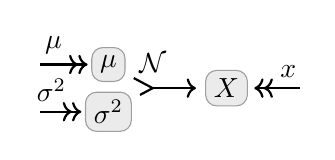
\begin{tikzpicture}[center base]
			\node[dpad0](X) at (0,0){$X$};
			% \node[dpad
			\draw[arr2, <<-] (X) to node[above,pos=0.7]{$x$} ++(1.0,0);
			% \draw[arr2, <-] (X) to node[above]{$\mathcal N(X|\mu,\sigma^2)$} ++(-1.7,0);
			\node[dpad0](m) at (-1.5, 0.3) {$\mu$};
			\node[dpad0](s2) at (-1.5, -0.3) {$\sigma^2$};
			\mergearr{m}{s2}{X};
			\node[above=2pt of center-ms2X](N){$\mathcal N$};
			\draw[arr1, <<-] (m) to node[above, pos=0.7]{$\mu$} +(-0.9,0);
			\draw[arr1, <<-] (s2) to node[above, pos=0.7]{$\sigma^2$} +(-0.9,0);
		\end{tikzpicture}}.
	\end{align*}

	The Fisher information for a normal distribution is given by
	\[
	\mathcal I(\mu, \sigma) =
	% \begin{bmatrix}
	%     \Ex_{\mathcal N(X|\mu,\sigma^2}[ \frac{\partial mathcal N(X|\mu,\sigma^2}{\partial \mu}) ]
	% \end{bmatrix}
	% =
	\begin{bmatrix}
		\frac1{\sigma^2} & 0 \\
		0 & \frac{1}{2 \sigma^4}
	\end{bmatrix}
	\]



	The natural gradient update rule is given by
	\begin{align*}
		F'_{x}(\mu, \sigma^2)
        &= - \hat\nabla_{\mu, \sigma^2} \mathcal L(x,\mu,\sigma^2)
        \\ &= \mathcal I(\mu, \sigma^2)^{-1}
		\begin{bmatrix}
			\frac{x-\mu}{\sigma} \\[1ex] \frac {-\sigma^2 + (x-\mu)^2}{2 \sigma^4}
		\end{bmatrix}
		=
		\begin{bmatrix}
			x-\mu \\ (x-\mu)^2 - \sigma^2
		\end{bmatrix}.
	\end{align*}

	Note that:
	\begin{itemize}
		\item  $\Ex_{x \sim \nu} [ F'_x(\mu,\sigma^2) ] = \mat 0$ if and only if $\nu$ has mean $\mu$ and variance $\sigma^2$.
		% We can interpret this in two ways:
		% This means that if observations are drawn from a fixed distribution $\nu(X)$,
		Moreover, this point is the unique global attractor.
		This means that,
		\begin{enumerate}
			\item If observations are drawn from a fixed distribution $\nu(X)$, and we repeatedly use $F$ to update $\theta = (\nu, \sigma)$ with small confidence $\epsilon$,
			then $\mu$ will approach the mean $\Ex_{\nu}[X]$ of $\nu$
			and $\sigma^2$ will approach the variance $\Ex_{\nu}[X^2] - \Ex_{\nu}[X]^2$.
			% If we make f observations are drawn from a fixed distribution $\nu(X)$,
			% If we update our belief parameters $\theta = (\mu, \sigma)$ according to $F$ with

			\item If we perform a single high-confidence update on the extended observation $\varphi \propto \nu$, in which each $x$ has relative confidence $\nu(x)$, the result will be a Gaussian with the mean and variance of $\nu$, i.e.,
			\[
				\forall \theta.\quad
				\lim_{c \to \infty} \Pr\nolimits_{F_{\nu}^c(\theta)} = \mathcal N(\Ex\nolimits_{\nu}[X], {\mathrm{Var}}_{\nu}[X])
			\]
		\end{enumerate}
		In this sense, relative confidence acts like probability.
		% So,

		\item
		If we update with the observation $x = \mu$ of our estimate with confidence $c$,
		the mean is unchanged, and our estimate of the variance becomes the harmonic mean of our previous variance $\sigma_0^2$ and the inverse confidence $\frac1c$.
		That is,
		\[
			F^c_\mu(\mu, \sigma_0^2) =
			\left(\mu, \frac{1}{c + \frac{1}{\sigma_0^2}} \right).
		\]
		Equivalently, the precision of the resulting distribution is the average of the confidence $c$ and the previous precision $\nicefrac{1}{\sigma_0^2}$, which suggests that confidence is of the same type as precision.
		%
		Note that if $\sigma_0^2$ is very large, so that our initial beliefs are very uncertain, updating with confidence $c$ results in variance $\frac1t$.
		In this sense, the magnitude of confidence acts as the inverse of variance.
	\end{itemize}
\end{example}


\section{Further Examples, in Depth}
\subsection{Update Rules for Discrete Probabilites}
\begin{table*}
\centering
\def\arraystretch{1.5}
\begin{tabular}{c|ccc|c}\toprule
    Dynamics $F$ & Flow $F^c_A(\mu)$
        & Vector Field $F'_A(\mu)$
        & Loss $\mathcal L^{F}(\mu, A)$
        & $F^c_A, F^{d}_B$ commute?
        \\\midrule
    $\mathit{LIN}$
        & $%\mathit{LIN}^c_A \mu =
            (1-c)\,\mu + (c)\,\mu| A$
        & $%\mathit{LIN}'_A \mu =
            \mu| A - \mu$
        & $%\mathcal L^{\mathit{LIN}}(\mu, A) =
            - \log \mu(A)$
        & if $\mu(A \cap B) > 0$
        \\[0.5ex]  %\noalign{\smallskip}
    $\mathit{LLI}$
        & {\def\arraystretch{0.8}
            \begin{tabular}{@{}l@{}}
            $\propto
                \mu^{1-c}\, (\mu|A)^c$\\
                \color{gray}
            $\propto
                \mu\, \mathbbm1_{A}$
            \end{tabular}}
        & {\color{red} N/A }
        & {\color{red} N/A }
        & always\\[1.5ex] %\noalign{\smallskip}
    $\mathit{Bolz}[\mathbf 1]$
        & {\def\arraystretch{0.9}\begin{tabular}{@{}l@{}}
            $\propto
                \mu \cdot \exp( \beta \mathbbm{1}_A)$\\
            \color{gray}
            $\propto
                \mu \cdot \exp( - \beta \mathbbm{1}_{\bar A})$
            \end{tabular}}
        & {\def\arraystretch{0.9}\begin{tabular}{@{}l@{}}
        	$\mu \odot (\mathbbm{1}_A - \mu(A))$\\
            \color{gray}
            $= \mu(A)\, (\mu|A - \mu)$ \\
			$= \mu \odot (\mathbbm{1}_A - \mu(A))$
            \end{tabular}}
        & $\mu(\lnot A)$
        & always \\
    \bottomrule
\end{tabular}
\caption{A comparison of different update rules when $\Theta = \Delta W$ and $\Phi = 2^W$}
\end{table*}


\begin{table*}
\centering
\begin{tabular}{c|ccc|c}\toprule
    Dynamics $F$ & Flow $F^c_q(\mu)$
        & Vector Field $F'_q(\mu)$
        & Loss $\mathcal L^{F}(\mu, q)$
        & Properties
        \\\midrule
    $\mathit{LIN}$
        & $%\mathit{LIN}^c_A \mu =
            (1-c)\,\mu + (c)\, q$
        & $%\mathit{LIN}'_A \mu =
            q - \mu$
        & $%\mathcal L^{\mathit{LIN}}(\mu, A) =
            \kldiv{q}{\mu}$
        & \\
    $\mathit{LLI}$
        & $\propto
            \mu^{1-c}\, q^c$
        & $\mu \odot \Big( \log \frac\mu q - \kldiv\mu q \Big)$
        & $\kldiv\mu q$
        &\\
    \bottomrule
\end{tabular}
\caption{Different update rules and their representations when $\Theta = \Phi = \Delta W$ }
\end{table*}

\subsection{Update Rules for Parametric Families}
\subsection{Kallman Filtering}

\section{Discussion}



\begin{contributions} % will be removed in pdf for initial submission,
                      % so you can already fill it to test with the
                      % ‘accepted’ class option
    Briefly list author contributions.
    This is a nice way of making clear who did what and to give proper credit.

    H.~Q.~Bovik conceived the idea and wrote the paper.
    Coauthor One created the code.
    Coauthor Two created the figures.
\end{contributions}

\begin{acknowledgements} % will be removed in pdf for initial submission,
                         % so you can already fill it to test with the
                         % ‘accepted’ class option
    Briefly acknowledge people and organizations here.

    \emph{All} acknowledgements go in this section.
\end{acknowledgements}

\ifbiblatex
    % \bibliography{uai2022-template}
    \printbibliography
\else
    \bibliography{conf}
\fi

\appendix
\onecolumn
\section{Discussion on Incremental Confidence and Independence Assumptions}

Historically, \cref{ax:funcform} has not proved as anodyne as it looks.
Some might object that it's not possible to write such a function that is appropriate in all circumstances.
For example, Shafer argues for Dempster's rule of combination as a way of incorporating information, but is very careful to emphasize that it ought to be used only on \emph{independent} information, for reasons illustrated below.



\begin{example}
    % \label{ex:dupl}
	You have initial belief state $\theta_0$.
	Now, someone comes up to you and tells you that $\phi$ is true, a statement
		that you trust to some intermediate degree of confidence $c \notin\{ \bot, \top\}$.
	So, in accordance with \Cref{ax:funcform}, you use $F$ to transform your beliefs, partially incorporating the information to arrive at some belief state $\theta_1 := F^c_\phi(\theta_0)$.
	Immediately afterwards, your friend repeats what they just said: $\phi$ is true.
	Your confidence in the statement remains the same, and so according to
	\Cref{ax:funcform}, you again update your beliefs, arriving at $\theta_2 := F^c_\phi(\theta_1)$.
	Except in very special circumstances (e.g., you already know that $\phi$ is true, or $c \in \{\bot,\top\}$), typically $\theta_2$.
	And yet, it seems your your attitude towards $\phi$ ought to be the same whether you've heard it twice or only once.
\end{example}


Now, it's important to mention that we're not quite in the same position as Shafer.
Shafer was prescribing a concrete representation of $\Theta$ (a belief function) and a concrete update rule $F$ (Dempster's rule of combination), and so he needed to defend these choices.
% To take an analogous prescriptive stance,
We only need to defend something much more modest: we only need to defend the assumption that, if $\Theta$ and $\Phi$ properly model the relevant aspects of the scenario at hand, then there exists \emph{some} function $F$ which performs updates appropriately.
Descriptively speaking, we're also in good shape: for synthetic agents, it suffices to point out that learning algorithms represent functions, which given a state, an input, and a number of iterations (confidence), produce an output.
And, supposing that $\Theta$, $\Phi$, and $\confdom$ all capture the relevant respective aspects of a human's belief state, input information, and attitude towards it, how could it be that a human does otherwise?
%
% After all, if you recieve the same input twice, and your confidence in it has not changed, it would be best to only update once.
% There are essentially three ways to proceed.
In any case, keeping \cref{ex:dupl} in mind, here are three ways to proceed.

\begin{enumerate}[label={\textbf{I\arabic*.}},ref={I\arabic*}]
	\item \textbf{Accept Severe Limiations.} \label{approach:assume}
	Like Shafer, we could be careful
	% not to claim anything about how to update beliefs, except
	to claim nothing about the belief updating process except in the (unusual) case where
	information recieved is independent.
	% This severly handicaps the usefulness of .
	This would be a severe limiation to the theory, and much less necessary than it was for Shafer.
	Imagine that we are writing code that describes how a synthetic agent updates its beliefs. Shafer's approach is to package any such code with a warning against running it unless assured that observations will always be independent.
	But independece is notoriously difficult to establish; are we to simply accept that the code will not behave correctly in any realistic scenario?
	% Under what circumstances could we possibly be sure that all inputs we will be independent?

	In practice, many theoretical properties of standard statistical learning algorithms are heavily dependent on indepencence assumptions (most commonly, that one recieves independent, identically distributed samples).
	% Despite this, such algorithms .
	This warning label not seem to keep them from being applied in settings where practitioners readily admit samples are not really independent at all---nor indeed performing well emperically in those settings \parencite{???}.

	% If we need to make a decision that depends on information that is not given, then
	% Shafer found himself in a position where he needed to qualify usage of the update rule


	\item \textbf{Appropriately Enrich Domains.}\label{approach:enrich}
	% For instace, the agent has been totally
	% We told a story wanting to avoid incorporating information twice.
	In \cref{ex:dupl}, it seems obvious that we ought to ignore the second copy of the information, because it has already been accounted for.
	However, this intuition is highly contingent on the implicit supposition that we \emph{know} the second input to be a replica of the first.
	Were we ignorant to the nature of the second piece of information, perhaps it would not be so unreasonable to incroproate it again, even without a proof of independence.
	% If we want our agent to do the same
	% In asking our agent to take such issues into account, it is only fair to give it access to the same
	% It seems unfair to criticize an agent for not behaving
	So, if we would like our agent to make the same decisions that we did, it seems only fair to give it access to the knowledge that we needed to get there.
	One way of doing this is to extend the belief state so that it also tracks what information has been incorporated.
	% For instance, suppose that every message

	For \cref{ex:dupl} to work, it is critical that we are able to discern that the two inputs were identical.
	As a result, it seems that the relevant description of the input information was not just $\phi$, but a pair $(\phi, \mathit{id})$ that also a description of its identity.
	It is also critical that we remember the identity of previously incorporated information, so we would also be better off with a belief space $\Theta$ reflects this.
	With these two modifications, any \cofunc\ can be straightforwardly modified to avoid the issue in \Cref{ex:dupl}.


	We submit that it is always possible to enrich the space of beliefs and observations in this way to track the relevant information, to resolve the issue.
	With a few more assumptions later on, we will be able to formalize the construction we just alluded to (\cref{ex:dupl-enriched}).

	\item \textbf{An Incremental Interpretation of Confidence.}
		\label{approach:interperet}
	Finally, we can get around the issue by interpreting a confidence $c \in \confdom$ not as an absolute measurement of confidence, but rather an incremental one.  This means viewing $c \in \confdom$ as the degree of \emph{additional} confidence we have in $\phi$, beyond whatever we have already incorporated into our beliefs.

	% This proposal immediately raises some important questions.
	This proposal might be concerning.
	% First, how
	One might worry that it's harder to make sense of ``incremental confidence'' than an absolute notion.
	How ought we to numerically describe the confidence of an update?
	Suddenly this becomes much more subjective, for to assign a number, not only must we describe how much trust we have in the new information, but we must also take history or current belief state into account.
	Furthermore, the words ``incremental'' and ``additional'' suggest that we will need a formal description of how to aggregate confidences---%
	the very concept of which we will need to defend.
	% Indeed, such a way of combining confidences will ultimately play a large role for us.
	% It will turn out that such a way of combining confidences
	% Fortunately, it will turn out that

	Even modulo these concerns, the incremental interpretation still leaves us in a strictly better place than we were before.
	%  with \cref{approach:assume}.
	To begin, in situations where inputs are independent (i.e., the only cases where we would have been allowed to apply the \cofunc\ according to \cref{approach:assume}), the two notions coincide.
	More explicitly: if the new information $\phi$ is indepenendent of everything we've previously seen, then an absolute measurement of our confidence in it is no different from a measrurement of how much we ought to increment it from having no confidence.
	Already, though, we can do more.
	In the situation described by \cref{ex:dupl}, for instance,
	the second utterance induce no \emph{additional} confidence ($\bot$), and so applying $F$ with no confidence clearly gives the desired result of ignoring the new information (per \cref{ax:zero}).
%
%
	And even in general, the prospect of having to numerically estimate a fuzzy quantity seems more promising than red tape requiring that $F$ only be used (in good conscience) on independent information.
	% In some ways, this approach it is not so different from directly requiring independence of inputs, there are several aspects of this framing, that in our view, make it more pallatable.
	% First,
	% In cases
	% This raises some questions. Even if we already had a

\end{enumerate}

We would like to point out that readers who find who find it reasonable to ignore inputs you have no confidence in (per \cref{ax:zero}) have implicitly either accepted either \cref{approach:assume} or \cref{approach:interperet}, as the next example shows. 


\begin{example}
	Suppose you first hear $\phi$ from a partially trusted source, and incroproate it into your beliefs appropriately.
	Then, the same source sends you a second message, which is obviously spam.
	In an absolute sense, you now have no confidence ($\bot$) in anything this source tells you, including (in retrospect) both messages.
	It seems appropriate to excise $\phi$ from your belief state in response, rather than leaving your belief state unchanged, as \cref{ax:zero} would prescribe.

	Note that in this scenario, while it seems that we ultimately have no confidence in $\phi$, it does not seem to be the case that we have no incremental confidence in $\phi$.
	Rather, the incremental confidence seems to be the inverse of the original confidence.
\end{example}

We state our results with the incremental interpretation of confidence, with the understanding that all of our results also admit a more conservative reading, in which confidence is measured absolutely, and also all applications of the function $F$ are independent. 

\section{Other Confidence Domains}

% \begin{phaseout}
To describe a degree of partial incorporation, we will need a domain of possible confidence values.
Mostly, we will stick to using real numbers, but it will clarify things to stay more general for now, so that we can see the properties we actually need.
% Formally, we represent the possible degrees of confidence by a group
Formally, a \emph{confidence domain} is a tuple $(\confdom, \oplus, \bot, \top)$,
where $(\confdom, \oplus, \bot)$ is a monoid with operation $\oplus$ and neutral element $\bot$, and $\top \in \confdom$ is an absorbing element---i.e., $\top \oplus c = \top$ for all $c \in \confdom$.
In terms of confidence, we interpret the components as follows:

\begin{itemize}%[]
	\item
	The elements of $\confdom$ are the possible degrees of confidence.

	\item
	The monoid operation $\oplus : \confdom \times \confdom \to \confdom$ describes how to combine two (independent) confidences in some statement, to obtain a new confidence in that statement.

	\item The neutral element $\bot \in \confdom$ indicates ``no confidence'' in an observation.
		%
		% The fact that we want to ignore information we have no confidence in
		% gives corresponds to the group identity laws: that
	The monoid identity laws, which assert that
		$\bot \oplus c = c = c \oplus \bot$ for all $c \in \confdom$,
	reflect the intuition that we should ignore untrusted information in combining confidences.
		% in which case we should ignore the information at hand,
	\item The absorbing element $\top$ indicates ``full confidence''.
	The absorbtion property corresponds to the intuition that, definitive information that $\phi$ is true, when combined with other (perhaps less reliable) information that $\phi$ is true, is still definitive.
\end{itemize}
% \end{phaseout}

In this more general setting, the analogue of additivity (\cref{ax:additivity}) becomes:
\begin{CFaxioms}
	\item For all $c_1, c_2 \in \confdom$,~
		% $F^{c_1}_\phi \circ F^{c_2}_\phi = F^{c_1 \oplus c_2}_\phi$
		$F^{c_1}_\phi \circ F^{c_2}_\phi = F^{c_1 \oplus c_2}_\phi$
		% \hfill \textbf{(additivity)} \label{ax:additivity}
		\hfill \textbf{(combination)} \label{ax:gen-combine}
\end{CFaxioms}
\Cref{ax:gen-combine}
 % looks like it could be problematic, but it
 simply states that \cofunc s respect the combination operation.
If we fix an assertion $\phi$, then an update with confidence $c_1$ followed by an update with confidence $c_2$ is equivalent to an update with confidence $c_1 \oplus c_2$, which is, by definition, the result of comining confidences $c_1$ and $c_2$.
On its own, so long as we have the freedom to choose $\confdom$, \Cref{ax:additivity} has no teeth.


\begin{prop} \label{prop:free-additivity}
	If $F: \confdom \to (\Phi \to (\Theta \to \Theta))$ satisfies \cref{ax:zero,ax:idemp}, then we can construct a new update
	% function for $\Theta$ on $\Phi$, that behaves in exactly the same way, but \emph{is} additive, but with the altered confidence domain
	function for $\Theta$ on $\Phi$, that behaves in exactly the same way, except that it is exteneded to a larger confidence domain, for which which it does satisfy \cref{ax:additivity}.
\end{prop}
\begin{lproof}
Consider the new confidence domain
$$
	\confdom' := \Big\{ \text{ finite lists } [c_1, \ldots c_n]
		\text{ with each } c_i \in \confdom,
		% \text{ such that } c_i \in \confdom \text{ for all } i = 1, \ldots, n
		\quad
		% \text{list concatenation}~::,
		::,
		\quad
		[\,],
		\quad
		[\top]
		\,
	\Big\},
$$
whose group operation ``$::$'' is list concatenation, except that it collapses instances of $\top$, i.e.,
\[
	[c_1, \ldots c_n] :: [d_1, \ldots, d_m]
	 := \begin{cases}
		 % [\top] & \text{ if } c_i = \top \text{ for some $i$ or $d_j=\top$ for some $j$}\\
		 [\top] & \text{ if } \top \in \{c_1, \ldots, c_n,d_1, \ldots,d_m \} \\
		 [c_1, \ldots, c_{n}, d_1, \ldots, d_m] & \text{otherwise.}
 \end{cases}
\]
Concatenating the empty list $[\,]$ on either side has no effect,
by construction, for all $L \in \confdom'$, we have $[\top] :: L = [\top] = L :: [\top]$,
and $::$ is clearly associative, so $\confdom'$ is also a confidence domain.

The new update rule for this confidence is given by:
	\[
		AF^{[c_1, \ldots, c_n]}_\phi (\theta)  :=
				(F^{c_n}_\phi \circ \cdots \circ F^{c_1}_\phi) (\theta).
	\]
$AF$ has the same behavior as $F$ on the elements that correspond to the original confidence domain, since
$
	AF^{[c]}_\phi(\theta) = F^c_\phi(\theta),
$
and it is additive by construction, since
\begin{align*}
AF^{[c_1, \ldots, c_n]}_\phi ( AF^{[d_1, \ldots, d_m]}_\phi (\theta) )
		&:=
			F^{d_m}_\phi \circ \cdots \circ F^{d_1}_\phi (
			F^{c_n}_\phi \circ \cdots \circ F^{c_1}_\phi (\theta))\\
		&= (F^{d_m}_\phi \circ \cdots \circ F^{d_1}_\phi \circ
		F^{c_n}_\phi \circ \cdots \circ F^{c_1}_\phi) (\theta) \\
		&= AF^{[c_1, \ldots, c_n, d_1, \ldots, d_m]}_\phi (\theta) \\
		&= AF^{[c_1, \ldots, c_n] :: [d_1, \ldots, d_m]}_\phi (\theta).
\end{align*}
\end{lproof}% We are primarily interested in the case where confidence can be measured as a real number,
For convenience of measurement, and so that we may better study confidence as a \emph{smooth} interpolation between ignoring and fully incorporation, we shall focus primarily on cases where confidence can be measured as a real number.
% We now define two confidence domains that are real numbers between 0 and 1.
We now consider two such confidence domains.

\begin{itemize}
	\item
	% Another confidence domain we could consider
	First, we consider the zero-one confidence domain
	\[
		\ZO := \Big(~ [0,1],
			% \quad a \star b := a b,
			\quad a \star b :=
					% 1- (1-a)(1-b) =
					a + b - ab,
			\quad 1,
			\quad 0 ~\Big),
	\]
	which uses the same numerical endpoints as probability;
	a value of zero represents no confidence, a value of one represents full confidence.
	For the purposes of updating, we may interpret a confidence of $a \in \ZO$ as the fration of the way between ignoring and fully incorporating information.
	This motivates the definition of the operator $\star$.
	If you go $90\%$ of the way to fully incorporaing some information $\phi$, and then $50\%$ of the remaining way, then in total you have gone $90\% + 50\%(100\%-90\%) = 0.9 + 0.5 - (0.9)(0.5)$ of the way to fully incorporating $\phi$.

	% In this domain
	% Clearly, 1 is neutral and 0 is absorbing element.\end{itemize}
	\item
	% First, we consider the monoid of positive extended real numbers under addition.
	We now introduce a second confidence domain based on the real numbers,
	which is mathematically cleaner, if
		% at first
		more difficult to interpret numerically in absolute terms.
	\[
		\Rplus :=
			\Big([0, \infty) \cup \{\infty\},
				\quad +,
				\quad 0,
				\quad \infty
				~\Big)
	\]

	% The use of addition as the combination operator means that independent measurements add, which in turn makes it
	The use of addition as the combination operator makes it particularly natural to speak of linear combinations of inputs.
	% Here are some examples.
	This point is best illustrated by example.

	\begin{itemize}
		\item \textbf{Voting.}
		Suppose the elements of $\Phi$ correspond to candidates in an election.
		In a sense, the number of votes a candidate recieves is a measure of how much confidence the electorate has in them---a candidate who recieves no votes is ignored, while a candidate who recieves all of the votes should be listened to exclusively.

		It's hard to say much  the raw number of votes a candidate recives in absolute terms, in part becasue it depends on the number of votes recieved by other candidates, and also how many votes you will recieve in the future.
		% Nevertheless, it is still m
		Nevertheless, if we are collecting votes, is especially natural to weight candidates by the total number of votes behind them.
		% Similarly, this way of counting fractional votes.
		This way of measuring confidence also applies without change to measure fractional votes.

		\item \textbf{Chemical Reactions.}
		Suppose that we have a mixture of nano-bots.
		Each nano-bot has some type $\phi \in \Phi$, and has the effect of turning matter into bots of type $\phi$.
		For every $\phi \in \Phi$, let $\beta_\phi$ be the concentration of bots of type $\phi$, say measured in number of bots per liter of solution.
		In some sense, $\beta_\phi$ measure of how much ``confidence'' the mixture has in $\phi$---if the concentration is zero, then that bot type may be ignored, and if all particles are of type $\phi$, then

		\TODO

		% Suppose that there is a chemical mixture of nano-bots. each of type $\phi_i$.

	\end{itemize}

	We will use greek letters $\alpha, \beta, \ldots$ to denote elements of $\Rplus$.

\end{itemize}


\begin{prop}
	$\ZO$ is isomorphic to $\Rplus$, but therere is no canonical choice of isomorphism.
\end{prop}
\begin{lproof}
	For every $k > 0$ can construct an isomorphism $\varphi_k: \ZO \to \Rplus$ explicitly by $\varphi(a) := - k \log a$.
	It is a homomorphism, since
	\[
		\varphi(a \star b) = - k \log (a b) = - k \log a - k \log b =
			\varphi(a) + \varphi(b),
	\]
	while $\varphi(1) = 0$ (so it preserves the identity) and $\varphi(0) = \infty$ (so it preserves the absorbing element).
	The inverse mapping can also be explicitly by $\varphi^{-1}(r) := \exp( - r / k)$, which is also a homorphism for the same reasons as above.
\end{lproof}


\section{Extra}

\subsection{Invertable Update Rules}

\begin{CFaxioms}
	\item For all $\phi\in\Phi$, and $\beta \in \mathbb R$, the update
	$F^{\beta}_{\phi}: \Theta \to \Theta$ is invertable.
	\hfill\textbf{(Invertability)} \label{ax:invert}
\end{CFaxioms}


This effectively partitions $\Theta$ into two


\begin{prop}
	If $F$ is a differentiable and invertable update rule (i.e., satisfies \cref{ax:zero,ax:additivity,ax:invert,ax:diffble}), then for all $\beta \in \mathbb R$, $\phi \in \Phi$, the function
	% $F^\beta_\phi : \Delta\X \to \Delta\X$
	$F^\beta_\phi : \Theta \to \Theta$
	is a diffeomorphism, and its inverse is given by $F^{-\beta}_\phi$, in the sense that
	\[
		F^{-\beta}_\phi( F^{\beta}_\phi (\mu) ) = \mu = F^{\beta}_\phi( F^{-\beta}_\phi (\mu) ).
	 \]
\end{prop}


% Together with strong additivity, we get
% \begin{prop% We are primarily interested in the case where confidence can be measured as a real number,
%     If $F$ is an update rule satisfying \cref{ax:additivity,ax:invert},
%     then any update prescribed by $F$ (or sequence thereof) takes positive distributions to positive distributions.
%     %
%     Concretely, for all $\beta$ and $\phi$,   $\mu \in \mathrm{Int}(\Delta\X)$ if and only if $F^{\beta}_\phi(\mu) \in \mathrm{Int}(\Delta\X)$.
%     If $F$ further satisfies \cref{ax:sufficiency, ax:diffble}, then
%     % \[
%         $F^\beta_\phi$ is a diffemorphism of $\mathrm{Int}(\Delta\X)$.
%     % \]
% \end{prop}


As a consequence,
\begin{coro}
	If for any $\beta < \infty$ there exist $\mu, \phi, A$ such that
	$\mu(A) > 0$  but $F^{\beta}_\phi(\mu)(A) = 0$, then $F$ is not invertable.
\end{coro}



\section{}
\begin{example}\label{ex:dupl-enriched}
Suppose $F$ is an additve update rule. Then, we can explicitly construct a resolution to the problem posed in \cref{ex:dupl} by defining enriched spaces
\begin{align*}
	\Phi' &:= \Phi \times \Big\{ \text{ identities }~ \mathit{id}~ \Big\}\\
	\Theta' &:= \Theta \times
		\Big\{ \text{histories } L = [(\phi_1, \mathit{id}_1, c_1), \ldots (\phi_n, \mathit{id}_n, c_n)] \Big\} \\
\end{align*}
and new \cofunc\ $G$ by
\begin{align*}
	 G^{\beta}_{(\phi,\mathit{id})}(\theta, L) & :=
		\begin{cases}
		\Big( F^{\beta- \sum_{i}\beta_i \mathbbm1[(\phi_i,\mathrm{id}_i) = (\phi, \mathrm{id})]}_{\phi}(\theta),~
			 L :: (\phi,\mathit{id}, \beta)
		 \Big)
			 &\text{ if } \beta \ne \bot \\
		(\theta, L) &
			   \text{ if } \beta = \bot
	\end{cases}
\end{align*}
\end{example}


\section{More on Path Update Rules}
Since each $\phi$ corresponds to a path

\begin{defn}[Homotopic update rules]
	$\phi \sim_F \psi$  iff 
	they behave the same way for full confidence (that is, 
	$F^1_{\phi}(\theta) = F^1_{\psi}(\theta)$ for all $\theta \in \Theta$)
	and  there exists a continuous function
	$H : \Theta \times [0,1] \times [0,1]$ such that,
	for all $\theta \in \Theta$ and $\chi \in [0,1]$,
	\begin{enumerate}[nosep]
		\item $H(\theta, \chi, 0)= F(\theta, \chi, \phi)$,
		\item $H(\theta, \chi, 1)= F(\theta, \chi, \psi)$
	\end{enumerate}
	and for all $s \in [0,1]$,
	\begin{enumerate}[nosep,resume]
		\item $H(\theta, 0, s) = \theta$;
		\item $H(\theta, 1, s) = F^1_{\phi}(\theta) = F^1_{\psi}(\theta)$,
		the last two of	which are the same by assumption. \qedhere
	\end{enumerate}
\end{defn}

As usual, homotopy is an equivalence relation.

For example, the Dempster-Shafer update rule \eqref{eq:ds-prob} is homotopic 
to the linear update rule from \cref{ex:prob-simple}. 


\section{Proofs}

\recall{theorem:add-reparam}
\begin{lproof}\label{proof:add-reparam}
    
\end{lproof}

\section{More Examples}


Next, and example in which we have an additive flow update rule,
that is not an optimizing update rule, and hence has no loss representation.

\begin{example}[Weighted Average]
    Suppose we recieve vectors $\phi \in \mathbb R^n$, 
    say estimates of a quantity from different sources.
    Suppose further that our belief state
    $(\mat x,w) \in \Theta$ consists a current estimate
    $\mat x$ of the quantity of interest, and a weight $w$ of the total internal confidence in the estimate.
    In other words:    
	\begin{align*}
		\Theta = \mathbb R^n \times [0,\infty];
		\qquad
        \text{and}
        \qquad
		\Phi = \mathbb R^n %; \qquad
        .
	\end{align*}

	Updating proceeds by taking a weighted average of the previous estimate and the new input, weighted by their respective confidences, which is captured by:
	\begin{align*}
		F^\beta_{\mat y}(\mat x, w) &=  \left( \frac{ w \mat x + \beta \mat y}{w + \beta} , w + \beta \right)
		\qquad\text{and}\qquad
		F^{\beta}_{\mat y}(\mat x, \infty) = (\mat x, \infty)
	\end{align*}
	It is additive, since
	\begin{align*}
		&F^{\beta_2}_{\mat y} \circ F^{\beta_1}_{\mat y}(\mat x, w) \\
		&= \left( \frac{ (w + \beta_1) \frac{ w \mat x + \beta_1 \mat y}{w + \beta_1} + \beta_2 \mat y}{(w + \beta_1) + \beta_2}, (w  + \beta_1) + \beta_2 \right) \\
		&= \left( \frac{  w \mat x + (\beta_1 + \beta_2) \mat y}{w + (\beta_1 + \beta_2)}, w  + (\beta_1 + \beta_2)\right)
		= F^{\beta_1 + \beta_2}_{\mat y}(\mat x, w).
	\end{align*}
	And it is clearly differentiable, with a simple calculation revealing that
	$ F'_{\mat y}(\mat x, w) = \left( \frac{\mat y - \mat x}{w}, 1\right) $.

	Observations:
	\begin{itemize}
		\item The update rule cannot be extended differentiably to states $\theta = (\mat x, w)$ with $w = 0$.
			Intuitively, we need to have some estimate with positive confidence to update beliefs in a differentiable way.
        This is related to the fact that plain emperical risk minimization (ERM) is unstable, but stable with even a small amount of regularization.
			% It is also similar to the fact that one needs a prior in order to do
			% In this case, the prior may be arbitrarily weak.
		\item The certainties are given by
		\[
			\lim_{\beta \to \infty} F^{\beta}_{\mat y}(\mat x, w) = (\mat y, \infty)
		\]
		% \item In this case,
		\item $F$ is commutative, invertible, and symmetric with respect to permutation of the dimensions, but it is not conservative: if we had $U(\mat x, w, \mat y)$ twice differentiable such that $\nabla_{\mat x, w} U = F'$, then we would have
        \begin{align*}
        \frac{\partial^2}{\partial w \partial x_i} U &=
			\frac\partial{\partial w} \frac{y_i - x_i}{w} = \frac{x_i - y_i}{w^2},\quad\text{but}
            \\
		\frac{\partial^2}{\partial x_1 \partial w} U
			&= \frac\partial{\partial x_i} 1 = 0    
        \end{align*}
		violating Clairaut's theorem (which asserts equality of mixed partials).
		Therefore, $F'$ cannot be written as the gradient of a function,
        and so $F$ is not an optimizing update rule. \qedhere
	\end{itemize}
\end{example}

Next, a toy example that showcases an assortment of other features and themes that can be captured with our definition of confidence.

\begin{example}\label{ex:jugo}
% \def\Gpressed(#1,#2){\mathsf{G}_{#1}\text{-}\mathit{pressed}(\mathsf{G},#1,#2)}
% \def\Gpressed(#1,#2){\mathit{pressed}(#1,\mathsf{G},#2)}
\def\pressed(#1,#2,#3){\mathit{pressed}(#1,\mathsf{#2},#3)}
Jugo is an impartial juror.
Like the other jurors, she has two buttons in front of her,
labeled $\sf G$ and $\sf N$.
% The button labeled $\mathsf G$ increases the probability 
% of a guilty verdict, while the button labeled $\mathsf N$ increases
% the probability of a not-guilty verdict. 
Her instructions are to listen to evidence, and press $\sf G$ to 
increase the probability of a guilty verdict, and $\sf N$ 
to increase the probability of a not-guilty verdict.

More concretely, the system works as follows.
There are $J$ jurors, labeled $\{1, \ldots, J\}$;
let 
% $G_j(t)$ be
$\pressed(j,B,t)$ be
a variable that is equal to one if juror $j \in $
is pressing button  $\mathsf B$ button at time $t$, and zero otherwise.
% ; symmetrically, let $N_j(t)$ indicate whether $j$ is pressing the $\mathsf N$ at time $t$.
The ``belief state'' of this automated system is
a single number $g \in [0,1]$, representing the probability of a guilty verdict.
When a single juror presses $\mathsf G$, $g$ approaches 1
exponentially, and if they instead press $\sf N$, $g$ decays to zero.
In the first case ($\sf G$ is pressed) the system evoves according to 
$\frac{\mathrm dg}{\mathrm dt} = (1-g)$
while in the second, 
$\frac{\mathrm dg}{\mathrm dt} = -g$.
The first is the vector field associated with the $\mathsf G$ button,
and the second is the vector field associated with $\sf N$. 
The total effect of all buttons is then the sum of that of all buttons across all vector fields, when they are active:
% in which case $g(t) = 1 + (g(0) - 1)e^{-t} $.
% Concretely, their dynamics are governed by:
\[
	\frac{\mathrm dg}{\mathrm dt} = 
	\sum_{j = 1}^J 
		% G_j(t)
		\pressed(j,G,t)
		(1-g) 
		-
		% N_j(t)
		\pressed(j,N,t)
		(g)
		~,
	% \begin{cases}
	% 	(1 - p)	& \text{button $\uparrow$ pressed} \\
	% 	-p & \text{button $\downarrow$ pressed}
	% \end{cases}	
\]
so that $g$ exponentially approahces $1$ when more $\mathsf G$ buttons are pressed than $\mathsf N$ buttons,
and symmetricaly, exponentially approaches $0$ when more $\mathsf N$ buttons than $\mathsf G$ buttons are pressed.
At the end of the trial, the defendant is convicted with probability
equal to the final value of $g$. 

Let $\phi$ represent a piece of evidence suggesting guilt, presented by the
prosecution from time $t_1$ to time $t_2$,
and suppose for now that only buttons labeled $\mathsf G$ are pressed
in this interval.
% Many aspects of this scenario can be understood in terms of confidence.
%
	% The amount of time that 
	% What is the confidence of the system in that evidence, as it understands it from the Jurors?
% First, suppose that only $\mathsf G$ buttons are pressed
	 % between $t_1$ and $t_2$. 
% in between times $t_1$ and $t_2$.
The system measures $j$'s confidence in $\phi$ by
\[
	w_j := \!\int_{t_1}^{t_2}\!\! G_j(t) \mathrm d t 
	= \text{ total time $j$ presses $\mathsf G$ during $\phi$,}
\]
Note that $w_j = 0$ if and only if $j$ does not press any buttons,
which (a) indicates that $j$ does not trust the evidence $\phi$, 
and (b) communicates this fact to the system, by telling it to ignore 
the evidence. 
Note that this is an additive representation of confidence, since
pressing the button for four seconds, and then three more later, is
by definition the same as pressing it for seven. 
While the maximum possible confidence of $w_j$ is $(t_2 - t_1)$,
this system does not allow a juror to express \emph{full} confidence in $\phi$
because no finite amount of $\mathsf G$-pressing will result in a 
guilty verdict with probability one; it is always possible to increase
the value of $g$ through additional evidence. 

% Now, recall that ,
Altogether, the system's confidence in $\phi$ can be measured by
as the unique value $W$ for which
\begin{align*}
	% \int_{t_1}^{t_2} W (1-g(t)) \mathrm d t = \int_{t_1}^{t_2} \sum_{j=1}^J G_j(t) (1-g(t)) \mathrm d t,
	\int_{t_1}^{t_2} W (1-g(t)) \mathrm d t =
	 g(t_2) - g(t_1),
	% \\
	% W = \frac{1}{t_2-t_1 - \int_{t_1}^{t_2}g(t) \mathrm dt} \int_{t_1}^{t_2} \sum_{j=1}^J G_j(t) (1-g(t)) \mathrm d t
\end{align*}
which, so long as only $\mathsf G$ buttons are pressed, equals
$W := \sum_{j} w_j$, so this measure of confidence is additive 
across jurors as well as across time. 
This is appropriate, since the jurors are independent and 
not communicating with each other.
% This is a weighted sum of $w_i's$
As before, $W = 0$ if and only if no juror presses any buttons between times $t_1$ and $t_2$,
indicating zero trust leant to $\phi$. In such a case, the system ignores $\phi$ in updating its beliefs.
And just as no individual juror can send a full-confidence update to the system,
	the system cannot recieve a full-confidence from the jurors as a whole.
	
The picture gets significantly more complicated if we consider the possibility
that jurors might press the $\mathsf N$ button. For example, if $\phi$, which was intended
as evidence of guilt, has the effect of getting jurors to press $\mathsf N$, there is a sense
in which they have \emph{negative} confidence in $\phi$, since the belief update happened in the opposite direction of what $\phi$ represents; rather than \emph{no} trust, this is represents \emph{distrust}. 
Small negative updates are always possible except at the boundary of belief space, but in this paper, we focus almost entirely on positive confidence updates.

The introduction of the second button also uncovers a significant source of complexity:
unlike \cref{ex:prob-simple,ex:classifier,ex:shafer}, 
the order that evidence is presented matters, when there is more than one possible response to it.
Evidence presented later has a larger effect,
meaning that this system exhibits a recency bias.
% (This lack of commutativity corresponds to possibility that,
%	as a Lie algebra, the bracket may not be identically zero.)

Now consider a variant of this system that does
not trust all jurors equally; rather, it trusts each juror $j$
to a degree $\beta_j \in [0, \infty]$, and now $g$ evolves
according to
\[
	\frac{\mathrm dg}{\mathrm dt} = 
	\sum_{j = 1}^J \beta_j \Big( G_j(t) (1-g) 
		- g N_j(t) \Big).
	% \begin{cases}
	% 	(1 - p)	& \text{button $\uparrow$ pressed} \\
	% 	-p & \text{button $\downarrow$ pressed}
	% \end{cases}	
\]
In this case, the system can be said to have trust $\beta_j$ in juror
$j$, since $j$'s buttons are ignored when $\beta_j = 0$. 
When $\beta_j = \infty$ (an expression of full confidence in $j$),
$g$ immediately jumps to 0 when $j$ presses 
$\mathsf N$, or to 1 if $j$ presses $\mathsf G$ (unless canceled by
another full-confidence juror pressing the opposite button).
If all jurors have full confidence, then the verdict of this system is
a majority vote at the last moment a button was pressed. 
Thus, the weights attached to weighted combinations are (additive) expressions 
of confidence as well. 
\end{example}

\section{Counter-Examples}

\subsection{Nonmonotonic Updates (Dropping \ref{ax:seq-for-more})}
    % strangely, doesn't work with \cref, or \ref* or \cref*.
Without \cref{ax:seq-for-more}, we could have a situation like the below,
in which resuming an update could take you to a completely different position
if you were interrupted in the middle of the path. 

\begin{center}
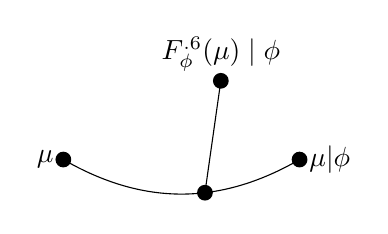
\begin{tikzpicture}
    \coordinate[label=left:$\mu$] (A) at (0,0);
    \coordinate[label=right:$\mu|\phi$] (C) at (3,0);
    \coordinate[label=above:$F_\phi^{.6}(\mu)\mid\phi$] (C') at (2,1);
    \draw (A) to[bend right] node[outer sep=0,pos=0.6](B){} (C);
    \fill 
        (A) circle (0.1)
        (B) circle (0.1)
        (C) circle (0.1)
        (C') circle (0.1);
    \draw (B.center) to (C');
\end{tikzpicture}
\end{center}


\subsection{Halting Updates (Dropping \ref{ax:nopause})}
The next two examples further explore the motivation behind \cref{ax:nopause}

\begin{example}
Suppose $\Theta = \mathbb R \cup \{-\infty, \infty\}$, $\Phi = \{\star\}$ is a singleton, and
and 
\[
    F^t_{\!\star}(\theta) = \theta + t + \sin(t).
\]

This is interesting because it ``pauses'' 
Clearly $F$ satisfies \cref{ax:zero,ax:idemp,ax:cont,ax:diffble}.
It also satisfies \cref{ax:seq-for-more}, since it is increasing in $t$
(but it is not additive \cref{ax:additivity}).
%
Its vector field is given by 
\[
    \frac{\partial}{\partial t} F^t_{\!\star}(\theta) = 1 + \cos(t) \Big|_{t=0}
     = 2,
\]
so its unique additive representation is
$
    {^+}F^t_{\!\star}(\theta) = \theta + 2 t.
$
\end{example}

\begin{example}
Now suppose $\Theta$ and $\Phi$ are as before,
but now
\[
    F^t_{\!\star}(\theta) = \theta + t - \sin(t).
\]
As before, it satisfies \cref{ax:zero,ax:idemp,ax:cont,ax:diffble,ax:seq-for-more},
but now its vector field is
\[
    \frac{\partial}{\partial t} F^t_{\!\star}(\theta) = 1 - \cos(t) \Big|_{t=0}
     = 0,
\]
so its unique additive representation does nothing:
$
    {^+}F^t_{\!\star}(\theta) = \theta. 
$
\end{example}

\subsection{}



\end{document}
